%&preformat-disser
\RequirePackage[l2tabu,orthodox]{nag} % Раскомментировав, можно в логе получать рекомендации относительно правильного использования пакетов и предупреждения об устаревших и нерекомендуемых пакетах
% Формат А4, 14pt (ГОСТ Р 7.0.11-2011, 5.3.6)
\documentclass[a4paper,14pt,oneside,openany]{memoir} %fleqn --- чтобы формулы были не по середине а слева

\input{common/setup}            % общие настройки шаблона
\input{common/packages}         % Пакеты общие для диссертации и автореферата
\synopsisfalse                      % Этот документ --- не автореферат
%%% Прикладные пакеты %%% 
%\usepackage{calc}               % Пакет для расчётов параметров, например длины

%%% Для добавления Стр. над номерами страниц в оглавлении
%%% http://tex.stackexchange.com/a/306950
\usepackage{afterpage}

\usepackage{tikz}                   % Продвинутый пакет векторной графики
\usetikzlibrary{chains}             % Для примера tikz рисунка
\usetikzlibrary{shapes.geometric}   % Для примера tikz рисунка
\usetikzlibrary{shapes.symbols}     % Для примера tikz рисунка
\usetikzlibrary{arrows}             % Для примера tikz рисунка
\ifnumequal{\value{imgprecompile}}{1}{% Только если у нас включена предкомпиляция
    \usetikzlibrary{external}   % подключение возможности предкомпиляции
    \tikzexternalize[prefix=Dissertation/images/] % activate! % здесь можно указать отдельную папку для скомпилированных файлов
    \ifxetex
        \tikzset{external/up to date check={diff}}
    \fi
}{}

% Мой шрифт для кода:
\usepackage{roboto}

% Шахматная доска
\usepackage[utf8]{inputenc}
\usepackage[english]{babel}
\usepackage{skak}

% Матан
\usepackage[T1]{fontenc}
\usepackage{amsmath}

\makeatletter
\newcommand*\rel@kern[1]{\kern#1\dimexpr\macc@kerna}
\newcommand*\widebar[1]{%
	\begingroup
	\def\mathaccent##1##2{%
		\rel@kern{0.8}%
		\overline{\rel@kern{-0.8}\macc@nucleus\rel@kern{0.2}}%
		\rel@kern{-0.2}%
	}%
	\macc@depth\@ne
	\let\math@bgroup\@empty \let\math@egroup\macc@set@skewchar
	\mathsurround\z@ \frozen@everymath{\mathgroup\macc@group\relax}%
	\macc@set@skewchar\relax
	\let\mathaccentV\macc@nested@a
	\macc@nested@a\relax111{#1}%
	\endgroup
}
\makeatother    % Пакеты для диссертации
\input{Dissertation/userpackages}   % Пакеты для специфических пользовательских задач

\input{Dissertation/setup}      % Упрощённые настройки шаблона

\input{common/newnames}         % Новые переменные, для всего проекта

\input{common/data}             % Основные сведения
\input{common/fonts}            % Определение шрифтов (частичное)
\input{common/styles}           % Стили общие для диссертации и автореферата
\input{Dissertation/disstyles}  % Стили для диссертации
\input{Dissertation/userstyles} % Стили для специфических пользовательских задач
%%% Библиография. Выбор движка для реализации %%%
\ifnumequal{\value{bibliosel}}{0}{%
    \input{biblio/predefined}   % Встроенная реализация с загрузкой файла через движок bibtex8
}{
    \input{biblio/biblatex}     % Реализация пакетом biblatex через движок biber
}

%%% Управление компиляцией отдельных частейs диссертации %%%
% Необходимо сначала иметь полностью скомпилированный документ, чтобы все
% промежуточные файлы были в наличии
% Затем, для вывода отдельных частей можно воспользоваться командой \includeonly
% Ниже примеры использования команды:
%
%\includeonly{Dissertation/part2}
%\includeonly{Dissertation/contents,Dissertation/appendix,Dissertation/conclusion}
%
% Если все команды закомментированы, то документ будет выведен в PDF файл полностью
\usepackage[utf8]{inputenc}
\usepackage{minted}
\usepackage{enumitem}
\usepackage{mathrsfs} % делает более красивым формулы. Почему?
\setlist[enumerate]{topsep=0pt,itemsep=-1ex,partopsep=1ex,parsep=1ex, leftmargin=17pt}

%%%% Чтобы текст не слипался с номером страницы (мое)
\geometry{footskip=1cm}

% Полезные команды для математики
\newcommand{\const}{\mathrm{const}}
\newcommand{\rang}{\mathop{\mathrm{rk}}}
\newcommand{\Tr}{\mathop{\mathrm{tr}}}
%\newcommand{\Tr}{\mathsf{Tr\,}}
\newcommand{\tsum}{\mathop{\textstyle\sum}\limits}
\newcommand{\tprod}{\mathop{\textstyle\prod}\limits}
\newcommand{\tvee}{\mathop{\textstyle\bigvee}\limits}
\newcommand{\twedge}{\mathop{\textstyle\bigwedge}\limits}
\newcommand{\diag}{\mathop{\mathrm{diag}}}
\newcommand{\argmin}{\mathop{\rm arg\,min}\limits}
\newcommand{\argmax}{\mathop{\rm arg\,max}\limits}
\newcommand{\sign}{\mathop{\rm sign}\limits}
\newcommand{\med}{\mathop{\rm med}\limits}
\newcommand{\SoftMax}{\mathop{\rm SoftMax}\nolimits}
\newcommand{\Dir}{\mathop{\rm Dir}\nolimits}

\renewcommand{\geq}{\geqslant}
\renewcommand{\leq}{\leqslant}
\newcommand{\ophi}{\phi}
\renewcommand{\phi}{\varphi}
\newcommand{\eps}{\varepsilon}
\newcommand{\kapa}{\varkappa}
\newcommand{\emset}{\varnothing}
\newcommand{\cond}{\mspace{3mu}{|}\mspace{3mu}}
\newcommand{\refuse}{\o}
\newcommand{\Loss}{\mathscr{L}}
\newcommand{\Expect}{\mathsf{E}}
\newcommand{\Disp}{\mathsf{D}}
\newcommand{\Var}{\mathsf{D}}

\def\RR{\mathbb{R}}
\def\DD{\mathbb{D}}
\def\cL{\mathscr{L}}
\def\cF{\mathscr{F}}
\def\cG{\mathscr{G}}
\def\cJ{\mathcal{J}}
\def\cN{\mathcal{N}}
\def\cB{\mathscr{B}}
\def\cK{\mathscr{K}}
\def\fF{\mathfrak{F}}
\def\fI{\mathfrak{I}}
\def\fM{\mathfrak{M}}

\newcommand{\what}{\widehat}
\newcommand{\wtil}{\widetilde}
\newcommand{\ttil}{\raisebox{0.2ex}{\tiny$\sim$}}
%\newcommand{\T}{\mathsf{T}}
\newcommand{\T}{\textsf{\upshape т}}
\newcommand{\phanT}{^{\vphantom{\T}}}
\newcommand{\ExpecT}{\Expect^{\phanT}}

% added by Evgeny Sokolov
\def\XX{\mathbb{X}}
\def\PP{\mathbb{P}}
\def\FF{\mathcal{F}}
\def\EE{\mathbb{E}}
\def\NN{\mathcal{N}}
\def\LL{\mathcal{L}}
\def\YY{\mathbb{Y}}
\def\AA{\mathcal{A}}
\newenvironment{esSolution}%
{\begingroup\par\noindent{\bf Решение.}}%
{\par\hfill$\scriptstyle\blacksquare$\medskip\endgroup}

\newcommand{\mat}[1]{\left(\begin{smallmatrix}#1\end{smallmatrix}\right)}

\newcommand{\KL}[2]{
	\text{KL}
	\left(\left.
	{#1}
	\mspace{3mu} \right\| \mspace{3mu}
	{#2}
	\right)
}

% Для табличек
\usepackage{booktabs}% http://ctan.org/pkg/booktabs
\newcommand{\tabitem}{~~\llap{\textbullet}~~}
\usepackage{graphicx}
\usepackage[table,xcdraw]{xcolor}

\begin{document}

\input{common/renames}                 % Переопределение именований

%%% Структура диссертации (ГОСТ Р 7.0.11-2011, 4)
% Титульный лист (ГОСТ Р 7.0.11-2001, 5.1)
\thispagestyle{empty}
\begin{center}
	{\textsc{ Федеральное государственное автономное образовательное учреждение высшего профессионального образования \\ Национальный исследовательский университет \\ «Высшая Школа Экономики»}}
\end{center}

%
\vspace{0pt plus2fill} %число перед fill = кратность относительно некоторого расстояния fill, кусками которого заполнены пустые места
\begin{center}
	{{\large \textsc{Факультет экономических наук}}}
\end{center}
%

%
\vspace{-20pt} %число перед fill = кратность относительно некоторого расстояния fill, кусками которого заполнены пустые места
\begin{center}
	{{\large \textsc{Образовательная программа «Экономика»}}}
\end{center}
%




\rule{16.5cm}{1.5pt}

\begin{center}
	{\Large{\so{\textsc{\textbf{КУРСОВАЯ  РАБОТА}}}} \\
		\vspace{10pt}
		\large{\textsc{Стохастические методы оптимизации}}}
\end{center}

\rule{16.5cm}{1.5pt}

%
\vspace{0pt plus4fill} %число перед fill = кратность относительно некоторого расстояния fill, кусками которого заполнены пустые места
\begin{flushright}
	\textsc{Выполнил: \\ студент группы БЭК1812 \\ Хайкин Глеб Алексеевич}
\end{flushright}

%
\vspace{0pt plus2fill} %число перед fill = кратность относительно некоторого расстояния fill, кусками которого заполнены пустые места
\begin{flushright}
\textsc{Научный руководитель: \\ cтарший преподаватель \\ Борзых Дмитрий Александрович}
\end{flushright}

%
\vspace{100pt}
	\begin{center}
		
\includegraphics[height=3cm]{images/logobcopy}
	\end{center}


%
\vspace{0pt plus4fill} %число перед fill = кратность относительно некоторого расстояния fill, кусками которого заполнены пустые места
{\centering \textsc{Москва \ "--- 2020}\par}

           % Титульный лист
\include{Dissertation/contents}        % Оглавление
\chapter*{Введение}                         % Заголовок
\addcontentsline{toc}{chapter}{Введение}    % Добавляем его в оглавление, если нет нумерации, то есть
%\chapter*{Введение}

\newcommand{\actuality}{}
\newcommand{\progress}{}
\newcommand{\aim}{{\textbf\aimTXT}}
\newcommand{\tasks}{\textbf{\tasksTXT}}
%\newcommand{\novelty}{\textbf{\noveltyTXT}}
\newcommand{\influence}{\textbf{\influenceTXT}}
\newcommand{\methods}{\textbf{\methodsTXT}}
\newcommand{\defpositions}{\textbf{\defpositionsTXT}}
\newcommand{\reliability}{\textbf{\reliabilityTXT}}
\newcommand{\probation}{\textbf{\probationTXT}}
\newcommand{\contribution}{\textbf{\contributionTXT}}
\newcommand{\publications}{\textbf{\publicationsTXT}}

%\input{common/characteristic} % Характеристика работы по структуре во введении и в автореферате не отличается (ГОСТ Р 7.0.11, пункты 5.3.1 и 9.2.1), потому её загружаем из одного и того же внешнего файла, предварительно задав форму выделения некоторым параметрам

%\textbf{Объем и структура работы.} Диссертация состоит из~введения, трёх глав,
%заключения и~двух приложений.
%% на случай ошибок оставляю исходный кусок на месте, закомментированным
%Полный объём диссертации составляет  \ref*{TotPages}~страницу
%с~\totalfigures{}~рисунками и~\totaltables{}~таблицами. Список литературы
%содержит \total{citenum}~наименований.
%
%Полный объём диссертации составляет
%\formbytotal{TotPages}{страниц}{у}{ы}{}, включая
%\formbytotal{totalcount@figure}{рисун}{ок}{ка}{ков} и
%\formbytotal{totalcount@table}{таблиц}{у}{ы}{}.   Список литературы содержит
%\formbytotal{citenum}{наименован}{ие}{ия}{ий}.

\noindent

\begin{figure}[!h]
	\centering
  \tikzset{every picture/.style={line width=0.75pt}} %set default line width to 0.75pt
  
  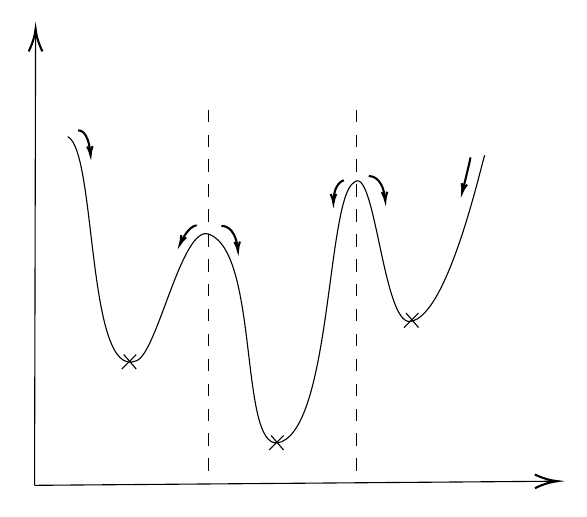
\begin{tikzpicture}[x=0.75pt,y=0.75pt,yscale=-1,xscale=1]
  %uncomment if require: \path (0,739); %set diagram left start at 0, and has height of 739

  %Curve Lines [id:da37232558430014473]
  \draw    (133.5,110) .. controls (158.5,119) and (147.5,219) .. (168.5,210) ;
  %Straight Lines [id:da3476897261424843]
  \draw    (49.5,231) -- (50,13) ;
  \draw [shift={(50,11)}, rotate = 450.13] [color={rgb, 255:red, 0; green, 0; blue, 0 }  ][line width=0.75]    (10.93,-3.29) .. controls (6.95,-1.4) and (3.31,-0.3) .. (0,0) .. controls (3.31,0.3) and (6.95,1.4) .. (10.93,3.29)   ;
  %Straight Lines [id:da355319366378235]
  \draw    (49.5,231) -- (299.5,229.02) ;
  \draw [shift={(301.5,229)}, rotate = 539.55] [color={rgb, 255:red, 0; green, 0; blue, 0 }  ][line width=0.75]    (10.93,-3.29) .. controls (6.95,-1.4) and (3.31,-0.3) .. (0,0) .. controls (3.31,0.3) and (6.95,1.4) .. (10.93,3.29)   ;
  %Curve Lines [id:da9451459693396738]
  \draw    (98.5,171) .. controls (108.5,168) and (120.5,105) .. (133.5,110) ;
  %Curve Lines [id:da9118683996504104]
  \draw    (168.5,210) .. controls (192.5,200) and (190.5,92) .. (203.5,85) ;
  %Curve Lines [id:da2198725124040073]
  \draw    (98.5,171) .. controls (74.5,181) and (79.5,70) .. (65.5,63) ;
  %Curve Lines [id:da7607618362532125]
  \draw    (230.5,152) .. controls (217.5,154) and (213.5,76) .. (203.5,85) ;
  %Curve Lines [id:da5694398882679776]
  \draw    (266.5,72) .. controls (266.5,68) and (249.5,150) .. (230.5,152) ;
  %Straight Lines [id:da9091864738783852]
  \draw  [dash pattern={on 4.5pt off 4.5pt}]  (133.5,50) -- (133.5,230) ;
  %Straight Lines [id:da6947024773973995]
  \draw  [dash pattern={on 4.5pt off 4.5pt}]  (204.5,50) -- (204.5,230) ;
  %Curve Lines [id:da3791802319426323]
  \draw [line width=0.75]    (70.5,60) .. controls (71.45,60) and (75.07,60) .. (76.31,70.13) ;
  \draw [shift={(76.5,72)}, rotate = 265.24] [color={rgb, 255:red, 0; green, 0; blue, 0 }  ][line width=0.75]    (4.37,-1.32) .. controls (2.78,-0.56) and (1.32,-0.12) .. (0,0) .. controls (1.32,0.12) and (2.78,0.56) .. (4.37,1.32)   ;
  %Curve Lines [id:da6195588467790258]
  \draw [line width=0.75]    (127.5,106) .. controls (128.45,106) and (124.92,104.21) .. (120.32,113.3) ;
  \draw [shift={(119.5,115)}, rotate = 294.44] [color={rgb, 255:red, 0; green, 0; blue, 0 }  ][line width=0.75]    (4.37,-1.32) .. controls (2.78,-0.56) and (1.32,-0.12) .. (0,0) .. controls (1.32,0.12) and (2.78,0.56) .. (4.37,1.32)   ;
  %Curve Lines [id:da14497801079245498]
  \draw [line width=0.75]    (139.5,106) .. controls (140.45,106) and (145.86,106) .. (147.29,116.13) ;
  \draw [shift={(147.5,118)}, rotate = 265.24] [color={rgb, 255:red, 0; green, 0; blue, 0 }  ][line width=0.75]    (4.37,-1.32) .. controls (2.78,-0.56) and (1.32,-0.12) .. (0,0) .. controls (1.32,0.12) and (2.78,0.56) .. (4.37,1.32)   ;
  %Curve Lines [id:da9889620169568767]
  \draw [line width=0.75]    (198.5,84) .. controls (199.44,84) and (194.19,84) .. (193.56,93.14) ;
  \draw [shift={(193.5,95)}, rotate = 270] [color={rgb, 255:red, 0; green, 0; blue, 0 }  ][line width=0.75]    (4.37,-1.32) .. controls (2.78,-0.56) and (1.32,-0.12) .. (0,0) .. controls (1.32,0.12) and (2.78,0.56) .. (4.37,1.32)   ;
  %Curve Lines [id:da9629769567992466]
  \draw [line width=0.75]    (210.5,82) .. controls (211.45,82) and (216.86,82) .. (218.29,92.13) ;
  \draw [shift={(218.5,94)}, rotate = 265.24] [color={rgb, 255:red, 0; green, 0; blue, 0 }  ][line width=0.75]    (4.37,-1.32) .. controls (2.78,-0.56) and (1.32,-0.12) .. (0,0) .. controls (1.32,0.12) and (2.78,0.56) .. (4.37,1.32)   ;
  %Curve Lines [id:da8600369809168591]
  \draw [line width=0.75]    (259.5,73) .. controls (259.5,73.87) and (257.23,83.07) .. (255.98,88.08) ;
  \draw [shift={(255.5,90)}, rotate = 284.04] [color={rgb, 255:red, 0; green, 0; blue, 0 }  ][line width=0.75]    (4.37,-1.32) .. controls (2.78,-0.56) and (1.32,-0.12) .. (0,0) .. controls (1.32,0.12) and (2.78,0.56) .. (4.37,1.32)   ;
  %Straight Lines [id:da8419867407870811]
  \draw    (92.5,168) -- (98.5,175) ;
  %Straight Lines [id:da60250082383082]
  \draw    (91.5,175) -- (98.5,168) ;
  %Straight Lines [id:da2923147725897497]
  \draw    (163.5,207) -- (169.5,214) ;
  %Straight Lines [id:da6189752522449852]
  \draw    (162.5,214) -- (169.5,207) ;
  %Straight Lines [id:da7981501034400449]
  \draw    (228.5,148) -- (234.5,155) ;
  %Straight Lines [id:da623222829834631]
  \draw    (227.5,155) -- (234.5,148) ;
  \end{tikzpicture}
	\label{img:example}
\end{figure}
    % Введение
\chapter{Имитация отжига} \label{SimulatedAnnealing}
\addcontentsline{toc}{chapter}{Имитация отжига}    % Добавляем его в оглавление, если нет нумерации
\noindent
\textit{Имитация отжига} (\emph{Simulated Annealing}, SA) представляет собой алгоритм решения задачи по поиску глобального оптимума некоторой функции~$F\colon \mathbb{X} \to \mathbb{R}$ через упорядоченный стохастический поиск, базирующийся на моделировании физического процесса кристализации вещества из жидкого состояние в твердое.

ДОБАВИТЬ ВВЕДНИЕ

\section{Алгоритм}

\noindent Для описания метода рассмотрим задачу нахождения глобального минимума:
\[
	F(x) \to \min \limits _{x \in \mathbb{X}},
\]

\noindent где~$x = (x_{1},\ldots , x_{m})$~--- вектор всех состояний, $\mathbb{X}$~--- множество всех состояний.

Положим, что~$k = 0$~и изначально температура зафиксированна на определенном уровне~$T(k) = const$.


\begin{enumerate}
	\item  Из множества всех состояний выберем случайный элемент~$\widehat{x}(k) \equiv x_i$,

	$i \in (1, ..., m)$.

	\item Понизим температуру одним из следующих способов:

		\begin{enumerate}
			\item Больцмановский отжиг
			\begin{equation}
			T(k) =  \dfrac{T(0)}{\ln (1 + k)}, \ k > 0
			\label{eq:boltzman}
			\end{equation}

			\item Отжиг Коши
			\begin{equation}
			T(k)  =  \dfrac{T(0)}{k}
			\end{equation}

			\item Метод тушения
			\begin{equation}
			T(k+1) = \alpha T(k),\ \alpha \in (0, 1)
			\end{equation}

		\end{enumerate}


	\item Пусть следующий элемент зависит от функции из семейства симметричных вероятностных распределений $G:$~$ \mathbb{X} \to \mathbb{X}$, порождающей новое состояние:
	\[
	\tilde{x}(k) \thicksim G(\widehat{x}(k), T(k)).
	\]

	\begin{enumerate}

		\item Часто G выбирается из семейства нормальных распределений:
		\begin{equation}
		\label{eq:normal_G}
		G(\tilde{x}; \widehat{x}, T)
		=
		\dfrac{1}
		{\sqrt{(2\pi)^{D} T}}
		\exp
		\left\lbrace
		\dfrac{- |\tilde{x} - \widehat{x}|^2}{2T}
		\right\rbrace,
		\end{equation}

		где $\widehat{x}$ — математическое ожидание, $T$  — дисперсия, $D$ — размерность пространства всех состояний.

		\item Также для D = 1 используется распределение Коши с плотностью:
		\begin{equation}
		G(\tilde{x}; \widehat{x}, T)
		=
		\dfrac{1}{\pi}
		\dfrac{T}{|\tilde{x}- \widehat{x}|^2 + T^2},
		\end{equation}

		где~$\widehat{x}$~--- параметр сдвига, $T$~--- параметр масштаба.





	\end{enumerate}

	\item Рассчитываем разницу двух функций:
	\[
	\Delta F =
	F(\tilde{x}(k))
	-
	F(\widehat{x}(k)).
	\]

	\item Принимаем~$\tilde{x}(k)$~за новый элемент, то есть~$\widehat{x}(k+1) \equiv \tilde{x}(k)$, с вероятностью
	\begin{equation}
	\mathbb{P}(\{\widehat{x}(k+1) = \tilde{x}(k)\})
	=
	\begin{cases}
	1,
	&
	\Delta F <0
	\\
	\exp
	\left\lbrace
	- \dfrac {\Delta F}{T(k)}
	\right\rbrace ,
	&
	\Delta F \geqslant 0
	\end{cases}
	\end{equation}

	и отвергаем его, то есть~$\widehat{x}(k+1) \equiv \widehat{x}(k)$, с вероятностью
	\[
	q
	=
	1 - \mathbb{P}(\{\widehat{x}(k+1) = \tilde{x}(k)\}).
	\]

	Заметим, чем выше температура, тем больше вероятность принять состояние хуже текущего ($\Delta F \geqslant 0$).

	\item Возвращаемся к пункту 2, пока не достигнем глобального минимума.

\end{enumerate}


%%%%%%%%%%%%%%%%%%%%%%%%%%%%%%%%%%%%%%%%%%%%%%%%%%%%%%%%%%%%%%%%%%%%%%%%%%%%%%%%%%%%%%%%%%%%%


\section{N ферзей}
\noindent Рассмотрим задачу, в которой необходимо расставить $N$ ферзей на шахматной доске размера $N \times  N$ так, чтобы ни один из них не <<бил>> другого.

В таком случае, множество всех состояний $\mathbb{X}$ будет содержать всевозможные расстановки ферзей на шахмотной доске. Общее число возможных расположений $n$ ферзей на $N \times N$-клеточной доске равно:
\[
{\begin{pmatrix} N \times N  \\ n \end{pmatrix}} = \dfrac{N \times N!}{n! (N \times N - n)!}
\]

Тогда  функция~$F:$~$\mathbb{X} \to \mathbb{R}$ будет выдавать количество атак ферзей, и решением данной задачи будет нахождение такого распложения~$x^{*}$, что~$F(x^*) \equiv 0$.

Зафиксируем изначальное расположение ферзей на шахматной доске. Очевидно, что несколько ферзей не могут находиться на одной вертикали или горизонтали, ибо тогда они будут находиться под ударом друг-друга. Следовательно, наша задача сужается к поиску расположения:
\begin{equation}
x* = (q_1, ..., q_n) = \{(1, h_1), ..., (n, h_n)\}, h_1 \neq ...  \neq h_n,
\end{equation}

где $(i, h_i)$ — расположение ферзя $q_i$ на i-ой вертикали по горизонтали $h_i$.

Отметим, что такая задача имеет $N!$ решений.

\newgame
\fenboard{q7/1q6/2q5/3q4/4q3/5q2/6q1/7q w - - 0 1}

\begin{figure}[h!]
	\begin{center}
		\showboard
		\legend{}
		\caption{ --- Изначальное расположение.}
		\label{img:nonopt}
	\end{center}
\end{figure}

Определим функцию, которая будет создавать изначальное неоптимальное расположение, в общем виде. Учитем, что несколько ферзей не могут находиться на одной вертикали или горизонтали.

\begin{pyin}
def queens(N):
  ver = np.arange(1, N + 1)
  hor = np.arange(1, N + 1)
  np.random.shuffle(hor)
  return np.column_stack((ver, hor)) # получаем массив
  # размерности (N, 2), отождествляющий расположение ферзей
\end{pyin}

Выведем первоначальное расположение ферзей для стандартной доски $8 \times 8$, где первый столбец массива — расположение по вертикали, второй столбец массива — расположение по горизонтали. Для наглядности — презентации оптимизационного процесса — выстроим изначальную расстановку на главной диагонали (рис. \ref{img:nonopt}).


\begin{pyin}
matrix = queens(8)
matrix
\end{pyin}

\begin{pyout}
array([[1, 1],
       [2, 2],
       [3, 3],
       [4, 4],
       [5, 5],
       [6, 6],
       [7, 7],
       [8, 8]])
\end{pyout}


Функция F, которая выявляет количество атак ферзей, выглядит следующим образом:
\begin{pyin}
def F(Q, N):
  cnt = 0
  for i in range(N):
     for j in range(i + 1, N):
         if abs(Q[i, 0] - Q[j, 0]) == abs(Q[i, 1] - Q[j, 1]):
             cnt += 1
  return cnt * 2 # учитываем взаимные атаки
\end{pyin}

Посмотрим, сколько у атак у исходной расстановки.
\begin{pyin}
F(matrix, 8)
\end{pyin}

\begin{pyout}
56
\end{pyout}

В нашей задачи функция G будет случайной незначительной перестановкой номеров горизонтали в исходном наборе.

\begin{pyin}
def G(Q, N):
  pos = Q.copy()
  while True:
     i = np.random.randint(0, N - 1)
     j = np.random.randint(0, N - 1)
     if i != j:
        break
  pos[i, 1], pos[j, 1] = pos[j, 1], pos[i, 1]
  return pos # получаем новое расположение
\end{pyin}

Теперь выведем и сам метод имитации отжига.

\begin{pyin}
def SA(Q, T, schedule):
  N = np.shape(Q)[0]
  x_hat = Q.copy()
\end{pyin}

\begin{pyprint}
  while F(x_hat, N) != 0:
     x_tilda = G(x_hat, N)
     delta = F(x_tilda, N) - F(x_hat, N)
     prob = np.exp(- delta / T)
     if (delta < 0) or (prob >= np.random.random()):
        x_hat = x_tilda
     # используем метод тушения для понижения температуры
     T *= schedule
  return x_hat
\end{pyprint}


\newgame
\fenboard{2q5/4q3/1q6/7q/q7/6q1/3q4/5q2 w - - 0 1}

\begin{figure}[h!]
	\begin{center}
		\showboard
		\legend{}
		\caption[р]{ --- Оптимальное расположение}
		\label{img:opt}
	\end{center}
\end{figure}


Так для нашего примера с гиперпараметрами $T(0) = 100, \alpha = 0.9$ мы получаем следующее оптимальное решение (рис. \ref{img:opt}):

\begin{pyin}
SA(matrix, 100, 0.9)
\end{pyin}

\begin{pyout}
array([[1, 4],
       [2, 6],
       [3, 8],
       [4, 2],
       [5, 7],
       [6, 1],
       [7, 3],
       [8, 5]])
\end{pyout}

\begin{figure}[h!]
\centering
\includegraphics [width=120mm]{queens8}
\caption{ --- Оптимизация расстановки 8 ферзей  в зависимости от гиперпараметра $\alpha$.}
\label{img:queens8}
\end{figure}

\begin{figure}[h!]
\centering
\includegraphics [width=120mm]{queens25}
\caption{ --- Оптимизация расстановки 25 ферзей  в зависимости от гиперпараметра $\alpha$.}
\label{img:queens25}
\end{figure}

\newpage

%%%%%%%%%%%%%%%%%%%%%%%%%%%%%%%%%%%%%%%%%%%%%%%%%%%%%%%%%%%%%%%%%%%%%%%%%%%%%%%%%%%%%%%%%%%%%


\section{Минимизация негладкой функции}

\noindent Воспользуемся алгоритмом имитации отжига для нахождения глобального минимума следующей функции:
\[
f(x) = x^2 (1 + |\sin 80x|).
\]

	\begin{figure}[h]
	\centering
	\includegraphics[width=120mm]{func_min}
	\caption{}
	\label{img:func_min}
\end{figure}

Стандартные методы оптимизации --- к примеру, метод градиентного спуска --- в данном случае не применимы. Вследствие наличия модуля этп функция не дифференцируема. Также она имеет очень большое количество локальных минимумов, что затрудняет, к примеру, мультистарт --- запуск градиентного спуска из разных начальных направлений.

Применим наш алгоритм к данной задачи. Пусть~$T(0) = 0.6$. Для понижения температуры будем использовать Больцмановский отжиг~(\ref{eq:boltzman}), а в качестве функции вероятностных распределений $G$ — семейство нормальных распределений~(\ref{eq:normal_G}).

\begin{pyin}
def SA(space, T, epsilon): # за space берется np.linspace(-2,2,1000)
  x_hat = np.random.choice(space)
  T_0 = T
  k = 1
  while True:
     x_tilda = np.random.normal(x_hat, T)
     delta = F(x_tilda) - F(x_hat)
     prob = np.exp(- delta / T)
\end{pyin}

\begin{pyprint}
     if (delta < 0) or (prob >= np.random.random()):
        x_hat = x_tilda
     if (x_hat < epsilon) and (x_hat > 0):
        return x_hat
     T = T_0 / np.log(1 + k)
     k += 1
\end{pyprint}

Остановка итерационного процесса и скорость метода зависят от того, насколько близко мы хотим приблизиться к глобальному минимуму. Так, при точности~$10^{-1}$, что довольно много, для 1000 повторений алгоритма метод отжига находит глобальный минимум в среднем за~1.97e-3~секунды со стандартным отклонением в~3.47e-5~секунды. Однако, увеличив точность до~$10^{-6}$, среднюю скорость занимает уже~1.27~секунды со стандартным отклонением в~2.1e-5~секунды. Это наглядно представлено на рисунке \ref{img:func_min1}.

\begin{figure}[h!]
	\centering
	\includegraphics[width=\linewidth]{func_min1}
	\caption{ --- Оптимизационный процесс в зависимости от точности.}
	\label{img:func_min1}
\end{figure}

\newpage

\section{Задача коммивояжера}

\noindent \emph{Задача коммивояжера} (\emph{Traveling Salesman Problem}, TSP) является образцовым методом проверки многих оптимизационных алгоритмов и заключается в поиске кратчайшего маршрута между городами. Путь должен быть проложен так, чтобы маршрут единственно проходил через все города и его конечная точка совпадала с  изначальной.

TSP имеет множество приложений в планировании и логистике, а также выступает в качестве подзадачи во многих других областях.  В таком случае города могут представлять, к примеру, клиентов, а расстояние между городами — время или стоимость путешествия.

\begin{figure}[h!]
\centering
\includegraphics [width=120mm]{TSP1}
\caption{ --- Изначальный маршрут для 26-ти городов.}
\label{img:tsp1}
\end{figure}

Для нашего примера создадим карту. Функция map\_city будет принимать желаемое количество городов в качестве входных данных и выдавать два списка, из которых далее создается общий список кортежей. Первым элементом кортежа является наименование города, а вторым --- его расположение в декартовой системе координат.

\begin{pyin}
def map_city(cities_num):
  letters = [chr(i) for i in range(65, 65 + cities_num)]
  coord = np.random.randint(1, 500, size=(cities_num, 2))
  return letters, coord
\end{pyin}

Наш маршрут будет состоять из 26-ти городов.

\begin{pyin}
names, cities = map_city(26)
store_val = list(zip(names, cities))
\end{pyin}


Определим расстояние от города i до всех остальных посредством функции distance\_dict. Для измерения расстояния между городами будем использовать евклидову метрику. Напомним, что евклидово расстояние между точками~$x = (x_1, ..., x_d)$~и~$u = (u_1, ..., u_d)$~задается как:
\[
\rho (x, u)
=
\sqrt{
\sum_{i = 1}^d \limits
(x_i - u_i)^2
}
\]

\begin{pyin}
def distance_dict(cities, n):
  d = dict()
  for i in range(n):
     city = dict()
     for j in range(n):
        if i == j:
           continue
        c_a = cities[i][1]
        c_b = cities[j][1]
        dist = np.sqrt((c_a[0] - c_b[0])**2 + (c_a[1] - c_b[1])**2)
        city[cities[j][0]] = dist
     d[cities[i][0]] = city
  return d
\end{pyin}


\begin{pyin}
cities_d = distance_dict(store_val, len(store_val))
\end{pyin}


Функция F для подсчета общего расстояния путешествия:

\begin{pyin}
def F(path, cities):
  dist = 0
  for i in range(len(path) - 1):
     dist += cities[path[i]][path[i + 1]]
  dist += cities[path[i + 1]][path[0]]
  return dist
\end{pyin}

За функцию G будет выступать простая перестановка как и в задаче о N ферзях.

\begin{pyin}
def G(path, n):
  pos = path.copy()
  while True:
     i = np.random.randint(0, n - 1)
     j = np.random.randint(0, n - 1)
     if i != j:
        break
     pos[i], pos[j] = pos[j], pos[i]
  return pos
\end{pyin}

\begin{figure}[h!]
\centering
\includegraphics [width=120mm]{TSP2}
\caption{ --- Применение метода отжига для построения оптимального маршрута для 26-ти городов.}
\label{img:tsp2}
\end{figure}


Для понижения температуры используем Больцмановский отжиг~(\ref{eq:boltzman}).

\begin{pyin}
def SA(path, T):
  path_hat = path
  n = len(path_hat)
  np.random.shuffle(path_hat)
  T_0 = T
  k = 1
  for i in range(100000):
     path_tilda = G(path_hat, n)
     delta = F(path_tilda, cities_d) - F(path_hat, cities_d)
\end{pyin}

\begin{pyprint}
     prob = np.exp(- delta / T)
\end{pyprint}

Теперь построим оптимальный маршрут (рис.~\ref{img:tsp2}).

\begin{pyin}
path_opt = SA(names, 100)
\end{pyin}

Несмотря на то, что метод отжига сократил преодалеваемую дистанцию, TSP была решена неидеально. К примеру, можно выделить соединение вершин E-S-L-V: очевидно, оно не оптимально, поскольку путь E-L-S-V имеет меньшее расстояние. Тем не менее, само расположение городов весьма удовлетворительно.

\section{Вывод}

\noindent
Рассмотрев метод отжига, выявим его плюсы и минусы.
\noindent
\begin{table}[h!]
	\caption{Метод отжига}
	\label{table:SA}
	\begin{tabular}{
	  p{\dimexpr.5\linewidth-2\tabcolsep-1.3333\arrayrulewidth}% column 1
	  p{\dimexpr.5\linewidth-2\tabcolsep-1.3333\arrayrulewidth}% column 2
	  }
	  \toprule
	  \centering Преимущества & \centering\arraybackslash Недостатки \\
		\midrule
	  1.~Имеет простую реализацию & 1.~Не подходит для задач с небольшим количеством локальных минимумов  \\[.5\normalbaselineskip]
		2.~Не застревает в локальных минимумах & 2.~Не всегда сходится к решению \\[.5\normalbaselineskip]
	  3.~Для сложных задач (наподобие TSP) дает вполне приемлемое решение &   \\[.5\normalbaselineskip]
		\bottomrule
	\end{tabular}
\end{table}

\chapter{Метод роения частиц} \label{ParticleSwarmOptimisation}
%\addcontentsline{toc}{chapter}{Метод роения частиц}    % Добавляем его в оглавление, если нет нумерации
\noindent
\emph{Метод роения частиц} (\emph{particle swarm optimization}, PSO) является одним из алгоритмов коллективной оптимизации и основывается на имитации социального поведения колониальных живых существ --- к примеру, колонии муравьев или стаи птиц, --- выполняющих коллективный поиск места с наилучшими условиями для существования.

Неформально данный алгоритм можно иллюстрировать следующем образом: при поиске пищи каждая особь передвигается по окружающей среде независимо от остальных членов колонии с некой долей случайности в своих движениях. Рано или поздно одна из особей находит пропитание и, будучи существом социальным, сообщает об этом остальным, что стягивает других к найденной пище.

\section{Алгоритм}
\noindent
Найдем глобальный экстремум функции~$F \colon \mathbb{R}^{n} \to \mathbb{R}$. Для определенности будем искать глобальный минимум:
\[
	\mathop{\mathrm{argmin}}_{x_i \in \mathbb{R}^{n}} F(x_i).
\]

Пусть в нашем рое $x$ существует~$\ell$~частиц размерности $\mathbb{R}^{n}$, тогда рой имеет вид~$x = \{x_i\}_{i = 1}^{\ell}$, где частица $x_i = (x_1, ..., x_n) \in D$.
$D = \{(x_1, ..., x_n) \in \mathbb{R}^n \ | \  a < x_i < b,\ \ a,\ b \in \mathbb{R} \}$ --- заданная область оптимизации (гиперкуб или гиперпрямоугольник).

Пусть также определен вектор скорости~$v = \{v_i\}_{i=1}^{\ell}$,~$i$-я компонента которого является скоростью~$i$-й частицы, $v_i = (v_1, ..., v_n) \in D$.

\begin{enumerate}
	\item Изначально случайным образом выбираем расположение роя $x_0$ и скорость движения каждой частицы $v_0$.

	\item Определяем новое расположение роя:
	\[
		x_{t + 1} \equiv x_t + v_t.
	\]

	\item Выбираем наилучшую точку для~$i$-й частицы:
	\begin{equation}
		\label{eq:personal_best}
		p_{i, t}
		=
		\begin{cases}
			x_{i, t},
			&
			F(x_{i, t + 1}) \geq F(x_{i, t})
			\\
			x_{i, t + 1},
			&
			F(x_{i, t + 1}) < F(x_{i, t})
		\end{cases}, \ i = 1, ..., \ell.
	\end{equation}

	Тогда вектор наилучших позиций для каждой частицы имеет вид:
	\[
		p_{t} = \{p_{i, t}\}_{i = 1}^{\ell}.
	\]

	\item Выбираем наилучшую точку для всего сообщества:
	\begin{equation}
		\label{eq:social_best}
		g_{t}
		\equiv
		\mathop{\mathrm{argmin}}_{i \in (1, ..., \ell)} \limits F(p_{i, t}).
	\end{equation}

	\item Обновляем скорость для~$i$-й частицы посредством следующей формулы:
	\begin{equation}
		\label{eq:new_velocity}
		v_{i, t + 1}
		\equiv
		w
		v_{i, t}
		+
		c_1
		\xi_{1, t}
		[p_{i, t} - x_{i, t}]
		+
		c_2
		\xi_{2, t}
		[g_{t} - x_{i, t}], \
		i = 1, ..., \ell,
	\end{equation}
	где $w \in \mathbb{R}$ --- инерционный вес,~$c_1,\ c_2 \in \mathbb{R}$ --- коэффициенты ускорения, $\xi_{1, t},\ \xi_{2, t} \sim U(0, 1)$.

	Тогда векотр скорости имеет вид:
	\[
		v_{t+1} = \{v_{i, t + 1}\}_{i = 1}^{\ell}.
	\]

	\vspace{10pt}

	\begin{figure}[!h]
	\centering
		\tikzset{every picture/.style={line width=0.75pt}} %set default line width to 0.75pt

		\begin{tikzpicture}[x=0.75pt,y=0.75pt,yscale=-1,xscale=1]
		uncomment if require: \path (0,429); %set diagram left start at 0, and has height of 429

		%Straight Lines [id:da4449765665231038]
		\draw    (182.83,365.09) -- (182.83,155.34) ;
		\draw [shift={(182.83,153.34)}, rotate = 450] [color={rgb, 255:red, 0; green, 0; blue, 0 }  ][line width=0.75]    (10.93,-4.9) .. controls (6.95,-2.3) and (3.31,-0.67) .. (0,0) .. controls (3.31,0.67) and (6.95,2.3) .. (10.93,4.9)   ;
		%Straight Lines [id:da7153141724618748]
		\draw [color={rgb, 255:red, 0; green, 0; blue, 0 }  ,draw opacity=1 ]   (182.83,365.09) -- (512.5,365.09) ;
		\draw [shift={(514.5,365.09)}, rotate = 180] [color={rgb, 255:red, 0; green, 0; blue, 0 }  ,draw opacity=1 ][line width=0.75]    (10.93,-3.29) .. controls (6.95,-1.4) and (3.31,-0.3) .. (0,0) .. controls (3.31,0.3) and (6.95,1.4) .. (10.93,3.29)   ;
		%Straight Lines [id:da049021320953235525]
		\draw [color={rgb, 255:red, 0; green, 0; blue, 0 }  ,draw opacity=1 ]   (182.83,365.09) -- (58.11,247.89) ;
		\draw [shift={(56.65,246.52)}, rotate = 403.22] [color={rgb, 255:red, 0; green, 0; blue, 0 }  ,draw opacity=1 ][line width=0.75]    (10.93,-3.29) .. controls (6.95,-1.4) and (3.31,-0.3) .. (0,0) .. controls (3.31,0.3) and (6.95,1.4) .. (10.93,3.29)   ;
		%Straight Lines [id:da20232334639948002]
		\draw [color={rgb, 255:red, 0; green, 0; blue, 0 }  ,draw opacity=1 ]   (182.83,365.09) -- (633.3,204.65) ;
		\draw [shift={(635.19,203.98)}, rotate = 520.4] [color={rgb, 255:red, 0; green, 0; blue, 0 }  ,draw opacity=1 ][line width=0.75]    (10.93,-3.29) .. controls (6.95,-1.4) and (3.31,-0.3) .. (0,0) .. controls (3.31,0.3) and (6.95,1.4) .. (10.93,3.29)   ;
		%Straight Lines [id:da30982294243702113]
		\draw  [dash pattern={on 4.5pt off 4.5pt}]  (183.71,29.64) -- (479.85,30.9) ;
		%Shape: Ellipse [id:dp3097132743634232]
		\draw  [color={rgb, 255:red, 255; green, 255; blue, 255 }  ,draw opacity=1 ][fill={rgb, 255:red, 0; green, 0; blue, 0 }  ,fill opacity=1 ] (518.98,362.76) .. controls (518.98,357.83) and (522.93,353.85) .. (527.8,353.85) .. controls (532.66,353.85) and (536.61,357.83) .. (536.61,362.76) .. controls (536.61,367.68) and (532.66,371.66) .. (527.8,371.66) .. controls (522.93,371.66) and (518.98,367.68) .. (518.98,362.76) -- cycle ;
		%Straight Lines [id:da6707373193501853]
		\draw  [dash pattern={on 4.5pt off 4.5pt}]  (645.14,199.17) -- (514.24,63.27) -- (479.85,30.9) ;
		%Shape: Ellipse [id:dp9920903593918595]
		\draw  [color={rgb, 255:red, 255; green, 255; blue, 255 }  ,draw opacity=1 ][fill={rgb, 255:red, 0; green, 0; blue, 0 }  ,fill opacity=1 ] (40.39,240.61) .. controls (40.39,235.68) and (44.34,231.7) .. (49.2,231.7) .. controls (54.07,231.7) and (58.02,235.68) .. (58.02,240.61) .. controls (58.02,245.53) and (54.07,249.51) .. (49.2,249.51) .. controls (44.34,249.51) and (40.39,245.53) .. (40.39,240.61) -- cycle ;
		%Shape: Ellipse [id:dp6112242856893209]
		\draw  [color={rgb, 255:red, 255; green, 255; blue, 255 }  ,draw opacity=1 ][fill={rgb, 255:red, 0; green, 0; blue, 0 }  ,fill opacity=1 ] (174.02,365.09) .. controls (174.02,360.17) and (177.96,356.18) .. (182.83,356.18) .. controls (187.7,356.18) and (191.65,360.17) .. (191.65,365.09) .. controls (191.65,370.01) and (187.7,374) .. (182.83,374) .. controls (177.96,374) and (174.02,370.01) .. (174.02,365.09) -- cycle ;
		%Shape: Ellipse [id:dp6835854741315035]
		\draw  [color={rgb, 255:red, 255; green, 255; blue, 255 }  ,draw opacity=1 ][fill={rgb, 255:red, 0; green, 0; blue, 0 }  ,fill opacity=1 ] (636.32,199.17) .. controls (636.32,194.25) and (640.27,190.26) .. (645.14,190.26) .. controls (650.01,190.26) and (653.95,194.25) .. (653.95,199.17) .. controls (653.95,204.09) and (650.01,208.07) .. (645.14,208.07) .. controls (640.27,208.07) and (636.32,204.09) .. (636.32,199.17) -- cycle ;
		%Straight Lines [id:da2902420192579651]
		\draw  [dash pattern={on 4.5pt off 4.5pt}]  (182.83,148.74) -- (182.79,29.64) ;

		% Text Node
		\draw (146,220.88) node [anchor=north west][inner sep=0.75pt]  [font=\normalsize]  {$v_{i,t}$};
		% Text Node
		\draw (375.46,269.9) node [anchor=north west][inner sep=0.75pt]  [font=\normalsize,rotate=-341.26,xslant=-0.03]  {$v_{i,t+1}$};
		% Text Node
		\draw (185,327) node [anchor=north west][inner sep=0.75pt]  [font=\normalsize]  {$x_{i,t}$};
		% Text Node
		\draw (610,209.67) node [anchor=north west][inner sep=0.75pt]  [font=\normalsize]  {$x_{i,t+1}$};
		% Text Node
		\draw (511.93,332) node [anchor=north west][inner sep=0.75pt]  [font=\normalsize]  {$p_{i,t}$};
		% Text Node
		\draw (62.39,222.19) node [anchor=north west][inner sep=0.75pt]  [font=\normalsize]  {$g_t$};
		% Text Node
		\draw (271.18,48.68) node [anchor=north west][inner sep=0.75pt]  [font=\normalsize,rotate=-359.87,xslant=0]  {$c_{1} \xi_{1,t}[p_{i,t} - x_{i,t}]$};
		% Text Node
		\draw (385.65,117.39) node [anchor=north west][inner sep=0.75pt]  [font=\normalsize]  {$c_{2} \xi _{2,t}[ g_t - x_{i,t}]$};
		% Text Node
		\draw (350.69,99.13) node [anchor=north west][inner sep=0.75pt]  [font=\normalsize] [align=left] {социальное воздействие};
		% Text Node
		\draw (252.05,31.73) node [anchor=north west][inner sep=0.75pt]  [font=\normalsize] [align=left] {когнитивное воздействие};
		% Text Node
		\draw (129.25,90.68) node [anchor=north west][inner sep=0.75pt]  [font=\normalsize]  {$wv_{i,t}$};
		% Text Node
		\draw (110,73.14) node [anchor=north west][inner sep=0.75pt]  [font=\normalsize] [align=left] {инерция};
		\end{tikzpicture}
	\vspace{-30pt}
	\caption{}
	\label{img:vectors}
	\end{figure}

	Три фактора влияют на частицу в положении $x_{i, t}$. С одной стороны, когнитивное воздействие побуждает частицу двигаться к ее лучшей позиции $p_{i, t}$, с другой стороны --- социальное воздействие побуждает частицу продвигаться в сторону лучшей позиции роя $g_{t}$. Кроме того, собственная скорость $v_{i, t}$ обеспечивает движение по инерции, что позволяет частице преодолевать локальные экстремумы и исследовать неизвестные области заданного пространства. Таким образом, происходит переход от точки $x_{i, t}$ в точку $x_{i, t+1}$ (рис. \ref{img:vectors}).

	PSO использует последовательности равномерно распределенных случайных величин~$\xi_{1, t},\ \xi_{2, t}$ и коэффициенты ускорения~$c_1,\ c_2$,опеределяющие максимальный размер шага, который частица может сделать за одну итерацию.	При~$c_1 = 0$~метод роения частиц будет опираться только на наилучшую позицию сообщества --- в таком случае алгоритм будет быстро сходиться, однако маловероятен факт нахождения глобального оптимума. При~$c_1 > 0$~метод использует связь всего сообщества --- скорость конвергенции падает, но глобальный оптимум оказывается более вероятным.

	\item Возвращаемся к пункту 2, пока не выполнен критерий останова.

	Приведем несколько примеров критерия останова:
	\begin{enumerate}
			\item Ограничить максимально возможное количество перемещений роя.
			\item Задать минимальную точность приближения.
			\item Определить минимальное уменьшение функции.
	\end{enumerate}


\end{enumerate}

\section{Функция Розенброка}
\label{section:rosenbrock}

\noindent
Функция Розенброка --- это невыпуклая функция вида
\[
	f(x_1, ..., x_n)
	=
	\sum^{n-1}_{i=1}\limits
	\left[
		(a - x_i)^2 + b(x_{i+1} - x^2)^2
	\rigth],
\]
использующаяся в качестве оценки производительности оптимизационных алоритмов. Для наших целей будем использовать трехмерный случай:
\[
	f(x, y) = (a - x)^2 + b(y-x^2)^2,
\]
где глобальный минимум достигается в точке $(a, a^2)$, где $f(a, a^2) = 0$.

\begin{figure}[ht]
	\centering
  \includegraphics[width=\linewidth]{rosenbrock}
  \caption{ --- Функция Розенброка с параметрами $a = 1$, $b = 100$.}
  \label{img:rosenbrock}
\end{figure}


Обычно $a = 1$, $b=100$. Тогда функция Розенброка примет следующий вид (рис. \ref{img:rosenbrock}):
\[
	f(x, y) = (1 - x)^2 + 100(y-x^2)^2.
\]

Глобальный минимум данной функции находится внутри так называемой <<долины>>: в нашем случае --- в точке $(1, 1)$. Приблизиться к долине легко, однако к глобальному минимуму --- довольно сложно.

Только при $a = 0$, функция является симметричной, а ее минимум находится в начале координат.

Определим функцию Розенброка:
\begin{pyin}
def func(x):
  return (1 - x[0]) ** 2 + 100 * (x[1] - x[0] ** 2) ** 2
\end{pyin}

Инициализируем метод роения частиц, используя объектно-ориентированное программирование. В первую очередь cоздадим класс частиц \texttt{Particle}. В нем зададим методы обновления позиции частицы \texttt{update\_position} и ее скорости \texttt{update\_velocity}. Также нам необходимо задать метод, который будет хранить наилучшую позицию частицы \texttt{choose\_personal\_best}.

\begin{pyin}
class Particle:
  def __init__(self, arg, space):
    # расположение частицы
    self.pos = np.asarray([])
    # вектор скорости частицы
    self.velocity = np.asarray([])
    # лучшее расположение частицы
		self.pos_best = None

    for i in range(arg):
       pos_i = np.random.uniform(space[i][0], space[i][1])
       self.pos = np.append(self.pos, pos_i)
       vel_i = np.random.uniform(0.2*space[i][0] , 0.2*space[i][1])
\end{pyin}

\begin{pyprint}
    self.velocity = np.append(self.velocity, vel_i)
    # список, состоящий из лучшего расположения частицы
    # и значения функции в данной точке
    self.pos_best = [self.pos.copy(), func(self.pos)]

  def update_position(self):
    self.pos += self.velocity

  def update_velocity(self, w, c1, c2, swarm_best):
    """
    INPUT:
    w --- инерционный вес
    c1 --- коэффициент ускорения когнитивного воздействия на частицу
    c2 --- коэффициент ускорения социального воздействия на частицу
    swarm_best --- лучшее расположение во всем рое
    """
    inertion = w * self.velocity
    xi_1 = np.random.uniform()
    xi_2 = np.random.uniform()
    cognitive_acceler = c1 * xi_1 * (self.pos_best[0] - self.pos)
    social_acceler = c2 * xi_2 * (swarm_best - self.pos)
    self.velocity = inertion + cognitive_acceler + social_acceler

  def choose_personal_best(self):
    if func(self.pos) < func(self.pos_best[0]):
       self.pos_best[0] = self.pos.copy()
       self.pos_best[1] = func(self.pos)
\end{pyprint}

Теперь cоздадим класс \texttt{ParticleSwarmOptimisation}. Определим методы \texttt{choose\_social\_best}, который выбирает лучшее расположение во всем рое, и \texttt{search\_global}, который реализует процесс оптимизации функции Розенброка.

\begin{pyin}
class ParticleSwarmOptimisation:
  def __init__(self, ell=40, w=1.0, c1=0.2, c2=0.2, max_iter=1000,
               tol=1e-24):
    """
    PARAMETERS:
    ell --- количество частиц в рое
    w --- инерционный вес
    c1 --- коэффициент ускорения когнитивного воздействия на частицу
    c2 --- коэффициент ускорения социального воздействия на частицу
    max_iter --- максимальное количество итераций
    tol --- минимальная точность
    """
\end{pyin}

\begin{pyprint}
    self.ell = ell
    self.w = w
    self.c1 = c1
    self.c2 = c2
    self.max_iter = max_iter
    self.tol = tol

    # лучшее расположение для всего роя
    self.swarm_best = None
    # расположение всех частиц (рой)
    self.swarm = None

  def search_global(self, arg, space):
    """
    INPUT:
    arg --- количество аргументов функции.
    space --- область поиска оптимума. Задается как список из
    кортежей, где кортеж --- это область значений
    одного аргумента функции.
    """
    self.arg = arg
    self.space = np.array(space)
    self.swarm = np.asarray([])

    # генерируем расположение роя
    for _ in range(self.ell):
       self.swarm = np.append(self.swarm,
                              Particle(self.arg, self.space))

    for k in range(self.max_iter):
       for i in range(self.ell):
          # обновляем расположение частицы
          self.swarm[i].update_position()
          # сравниваем с лучшей точкой частицы
          self.swarm[i].choose_personal_best()

       # выбираем лучшую точку для роя
       if k != 0:
          dist_0 = self.dist(self.swarm_best[0])
          self.choose_social_best()
          dist_1 = self.dist(self.swarm_best[0])

          # останавливаем поиск в условиях заданной точности
          if (dist_0 != dist_1) and (abs(dist_0-dist_1) <= self.tol):
             break
\end{pyprint}

\begin{pyprint}
          else:
             self.choose_social_best()

       # обновляем вектор скорости
       for i in range(self.ell):
          self.swarm[i].update_velocity(self.w, self.c1,
                                        self.c2, self.swarm_best[0])

    print(f"Глобальный оптимум: {self.swarm_best[0]}")
    print(f"Значение функции в данной точке: {self.swarm_best[1]}")

  def choose_social_best(self):
    best = min([[self.swarm[i].pos_best[0],
                 self.swarm[i].pos_best[1]] for i in range(self.ell)],
                 key=lambda x: x[1])
    self.swarm_best = best

  def dist(self, x):
    return np.sqrt(np.sum(x ** 2))
\end{pyprint}

 Инерционный вес \texttt{w} должен быть близким к $1$, а коэффициенты ускорения \texttt{c1}, \texttt{c2} --- достаточно малыми. Это дает возможность каждой случайно перемещающейся частице как можно обширнее исследовать заданное пространство, постепенно сходясь к наилучшему положению роя. Исходя из этого, мы устанавили по умолчанию именно такие гиперпараметры: \texttt{w=1.0}, \texttt{c1=0.2}, \texttt{c2=0.2}.

Реализуем PSO на функции Розенброка. Рой будет содержать 100 частиц. Зададим вес \texttt{w=0.95}.
\begin{pyin}
swarm_optimizer = ParticleSwarmOptimisation(w=0.95, ell=100)
\end{pyin}

Найдем глобальный минимум заданной функции. Перемещение роя в поисках глобального оптимума представлено на рисунке \ref{img:swarm}.
\begin{pyin}
np.random.seed(53)
swarm_optimizer.search_global(2, [(-10, 10),(-10, 10)])
\end{pyin}

\begin{pyout}
Глобальный оптимум: [1. 1.].
Значение функции в данной точке: 6.366439023928984e-22.
\end{pyout}

\begin{figure}[h!]
\centering
\includegraphics[width=\linewidth]{swarm}
\caption{ --- Расположение роя в разные моменты времени.}
\label{img:swarm}
\end{figure}

\begin{figure}[h!!]
\centering
\includegraphics[width=\linewidth]{PSO}
\caption{ --- Оптимизационный процесс.}
\label{img:PSO}
\end{figure}

За 1000 итераций метод роения частиц сходится к глобальному минимуму функции Розенборока с экспоненциальной скоростью с очень высокой точностью в 6.37e-22 (рис.\ref{img:PSO}). Средняя скорость реализации алгоритма составляет 1.79 секунды со стандартным отклонением в 0.111 секунд.


\section{Вывод}

\noindent
Рассмотрев метод роения частиц, выявим его плюсы и минусы.
\noindent
\begin{table}[h!]
	\caption{Метод роения частиц}
	\label{table:PSO}
	\begin{tabular}{
	  p{\dimexpr.5\linewidth-2\tabcolsep-1.3333\arrayrulewidth}% column 1
	  p{\dimexpr.5\linewidth-2\tabcolsep-1.3333\arrayrulewidth}% column 2
	  }
	  \toprule
	  \centering  Преимущества & \centering\arraybackslash  Недостатки \\
		\midrule
	  1.~Не требует дифференцируемости и непрерывности исследуемой функции &  \\[.5\normalbaselineskip]
		2.~Не застревает в локальных экстремумах &   \\[.5\normalbaselineskip]
	  3.~Находит глобальный экстремум с очень высокой точностью &   \\[.5\normalbaselineskip]
		\bottomrule
	\end{tabular}
\end{table}

\chapter{Генетический алгоритм} \label{ParticleSwarmOptimisation}
%\addcontentsline{toc}{chapter}{Метод роения частиц}    % Добавляем его в оглавление, если нет нумерации
\noindent
\emph{Генетический алгоритм} (\emph{Genetic Algorithm}, GA) является одним из самых популярных типов эволюционных алгоритмов, которые — как можно понять из их названия, — используют теорию эволюции, в частности теорию Дарвина, в решении той или иной оптимизационной задачи. Суть алгортима заключается в поиске наилучшего решения по принципу естественного отбора: случайным образом создается поколение, в ходе эволюции которого происходит скрещевание генов --- таким образом, появлется новое поколение (старые особи создают потомков) --- и их мутация.

\section{Алгоритм}
\noindent
Традиционно в качестве решения генетический алгоритм использует бинарное кодирование (binary encoding). Однако в данной работе будет проиллюстрирован метод реального кодирования (real value encoding), то есть решение будет представляться в вещественных числах.

Рассмотрим задачу нахождения глобального минимума функции~$F \colon \mathbb{R}^n \to \mathbb{R}$:
\[
	\mathop{\mathrm{argmin}}_{x \in \mathbb{R}^n}f(x),
\]
где каждая особь кодируется вектором $x = (x_1, ..., x_n)$, называемым хромосомой, компоненты которого являются генами.

\begin{figure}[!h]
\centering
\tikzset{every picture/.style={line width=0.75pt}} %set default line width to 0.75pt

\begin{tikzpicture}[x=0.75pt,y=0.75pt,yscale=-1,xscale=1]
%uncomment if require: \path (0,739); %set diagram left start at 0, and has height of 739

%Shape: Rectangle [id:dp8612057014709158]
\draw   (80,71) -- (110.5,71) -- (110.5,100) -- (80,100) -- cycle ;
%Shape: Rectangle [id:dp9416262412972431]
\draw   (110.5,71) -- (141,71) -- (141,100) -- (110.5,100) -- cycle ;
%Shape: Rectangle [id:dp9259667143051737]
\draw   (141,71) -- (171.5,71) -- (171.5,100) -- (141,100) -- cycle ;
%Shape: Rectangle [id:dp4285081026342692]
\draw   (171.5,71) -- (202,71) -- (202,100) -- (171.5,100) -- cycle ;
%Shape: Rectangle [id:dp6066867188861804]
\draw   (202,71) -- (232.5,71) -- (232.5,100) -- (202,100) -- cycle ;
%Curve Lines [id:da8858061911822572]
\draw    (232.5,71) .. controls (289.5,72) and (230.5,126) .. (308.5,126) ;
%Straight Lines [id:da05811670243584288]
\draw    (158.5,45) -- (158.5,68) ;
\draw [shift={(158.5,70)}, rotate = 270] [color={rgb, 255:red, 0; green, 0; blue, 0 }  ][line width=0.75]    (10.93,-3.29) .. controls (6.95,-1.4) and (3.31,-0.3) .. (0,0) .. controls (3.31,0.3) and (6.95,1.4) .. (10.93,3.29)   ;
%Shape: Rectangle [id:dp4349277402828884]
\draw   (81,151) -- (111.5,151) -- (111.5,180) -- (81,180) -- cycle ;
%Shape: Rectangle [id:dp24027028194138378]
\draw   (111.5,151) -- (142,151) -- (142,180) -- (111.5,180) -- cycle ;
%Shape: Rectangle [id:dp0500263413916362]
\draw   (142,151) -- (172.5,151) -- (172.5,180) -- (142,180) -- cycle ;
%Shape: Rectangle [id:dp8133255101181311]
\draw   (172.5,151) -- (203,151) -- (203,180) -- (172.5,180) -- cycle ;
%Shape: Rectangle [id:dp367355050028054]
\draw   (203,151) -- (233.5,151) -- (233.5,180) -- (203,180) -- cycle ;
%Curve Lines [id:da7627402544422663]
\draw    (233.5,180) .. controls (290.5,181) and (230.5,126) .. (308.5,126) ;
%Shape: Circle [id:dp7594178378532763]
\draw   (113.75,165.5) .. controls (113.75,158.32) and (119.57,152.5) .. (126.75,152.5) .. controls (133.93,152.5) and (139.75,158.32) .. (139.75,165.5) .. controls (139.75,172.68) and (133.93,178.5) .. (126.75,178.5) .. controls (119.57,178.5) and (113.75,172.68) .. (113.75,165.5) -- cycle ;
%Straight Lines [id:da7888876982561981]
\draw    (161.5,202) -- (131.49,175.33) ;
\draw [shift={(130,174)}, rotate = 401.63] [color={rgb, 255:red, 0; green, 0; blue, 0 }  ][line width=0.75]    (10.93,-3.29) .. controls (6.95,-1.4) and (3.31,-0.3) .. (0,0) .. controls (3.31,0.3) and (6.95,1.4) .. (10.93,3.29)   ;

% Text Node
\draw (80,122) node [anchor=north west][inner sep=0.75pt]   [align=left] {..............................};
% Text Node
\draw (311,120) node [anchor=north west][inner sep=0.75pt]  [font=\small] [align=left] {Популяция};
% Text Node
\draw (123,30) node [anchor=north west][inner sep=0.75pt]  [font=\small] [align=left] {Хромосома};
% Text Node
\draw (85,78) node [anchor=north west][inner sep=0.75pt]  [font=\small] [align=left] {$\displaystyle x_{11}$};
% Text Node
\draw (146,78) node [anchor=north west][inner sep=0.75pt]  [font=\small] [align=left] {$\displaystyle x_{13}$};
% Text Node
\draw (207,78) node [anchor=north west][inner sep=0.75pt]  [font=\small] [align=left] {$\displaystyle x_{1n}$};
% Text Node
\draw (115.5,78) node [anchor=north west][inner sep=0.75pt]  [font=\small] [align=left] {$\displaystyle x_{12}$};
% Text Node
\draw (179,82) node [anchor=north west][inner sep=0.75pt]   [align=left] {...};
% Text Node
\draw (86,158) node [anchor=north west][inner sep=0.75pt]  [font=\small] [align=left] {$\displaystyle x_{\ell 1}$};
% Text Node
\draw (147,158) node [anchor=north west][inner sep=0.75pt]  [font=\small] [align=left] {$\displaystyle x_{\ell 3}$};
% Text Node
\draw (208,158) node [anchor=north west][inner sep=0.75pt]  [font=\small] [align=left] {$\displaystyle x_{\ell n}$};
% Text Node
\draw (116.5,158) node [anchor=north west][inner sep=0.75pt]  [font=\small] [align=left] {$\displaystyle x_{\ell 2}$};
% Text Node
\draw (180,162) node [anchor=north west][inner sep=0.75pt]   [align=left] {...};
% Text Node
\draw (163.5,205) node [anchor=north west][inner sep=0.75pt]  [font=\small] [align=left] {Ген};
\end{tikzpicture}
\caption{}
\end{figure}

Пусть у нашего поколения, или популяции, $P$ есть $\ell$ особей. Тогда поколение в момент времени $t$ примет следующий вид:
\[
	P_t = \{x_{i,t}\}_{i=1}^\ell,
\]
где у кажой хромосомы имеется $n$ генов: $x_{i, t} = (x_{i1,t}, ..., x_{in, t})$

\begin{figure}[!h]
	\centering


	\tikzset{every picture/.style={line width=0.75pt}} %set default line width to 0.75pt

	\begin{tikzpicture}[x=0.75pt,y=0.75pt,yscale=-1,xscale=1]
	%uncomment if require: \path (0,739); %set diagram left start at 0, and has height of 739


	%Rounded Rect [id:dp6834144691063508]
	\draw  [color={rgb, 255:red, 128; green, 128; blue, 128 }  ,draw opacity=1 ][fill={rgb, 255:red, 155; green, 155; blue, 155 }  ,fill opacity=0.06 ] (240.5,57) .. controls (240.5,48.16) and (247.66,41) .. (256.5,41) -- (474.5,41) .. controls (483.34,41) and (490.5,48.16) .. (490.5,57) -- (490.5,105) .. controls (490.5,113.84) and (483.34,121) .. (474.5,121) -- (256.5,121) .. controls (247.66,121) and (240.5,113.84) .. (240.5,105) -- cycle ;
	%Rounded Rect [id:dp6349764616806755]
	\draw   (400.5,316) .. controls (400.5,307.16) and (407.66,300) .. (416.5,300) -- (634.5,300) .. controls (643.34,300) and (650.5,307.16) .. (650.5,316) -- (650.5,364) .. controls (650.5,372.84) and (643.34,380) .. (634.5,380) -- (416.5,380) .. controls (407.66,380) and (400.5,372.84) .. (400.5,364) -- cycle ;
	%Rounded Rect [id:dp3411925739284387]
	\draw   (79.5,316) .. controls (79.5,307.16) and (86.66,300) .. (95.5,300) -- (313.5,300) .. controls (322.34,300) and (329.5,307.16) .. (329.5,316) -- (329.5,364) .. controls (329.5,372.84) and (322.34,380) .. (313.5,380) -- (95.5,380) .. controls (86.66,380) and (79.5,372.84) .. (79.5,364) -- cycle ;
	%Rounded Rect [id:dp15356651288080547]
	\draw  [color={rgb, 255:red, 128; green, 128; blue, 128 }  ,draw opacity=1 ][fill={rgb, 255:red, 155; green, 155; blue, 155 }  ,fill opacity=0.06 ] (241.5,187) .. controls (241.5,178.16) and (248.66,171) .. (257.5,171) -- (475.5,171) .. controls (484.34,171) and (491.5,178.16) .. (491.5,187) -- (491.5,235) .. controls (491.5,243.84) and (484.34,251) .. (475.5,251) -- (257.5,251) .. controls (248.66,251) and (241.5,243.84) .. (241.5,235) -- cycle ;
	%Rounded Rect [id:dp13735168020488797]
	\draw  [color={rgb, 255:red, 128; green, 128; blue, 128 }  ,draw opacity=1 ][fill={rgb, 255:red, 155; green, 155; blue, 155 }  ,fill opacity=0.06 ] (400.5,316) .. controls (400.5,307.16) and (407.66,300) .. (416.5,300) -- (634.5,300) .. controls (643.34,300) and (650.5,307.16) .. (650.5,316) -- (650.5,364) .. controls (650.5,372.84) and (643.34,380) .. (634.5,380) -- (416.5,380) .. controls (407.66,380) and (400.5,372.84) .. (400.5,364) -- cycle ;
	%Rounded Rect [id:dp18159494190384895]
	\draw  [color={rgb, 255:red, 128; green, 128; blue, 128 }  ,draw opacity=1 ][fill={rgb, 255:red, 155; green, 155; blue, 155 }  ,fill opacity=0.06 ] (240.5,446) .. controls (240.5,437.16) and (247.66,430) .. (256.5,430) -- (474.5,430) .. controls (483.34,430) and (490.5,437.16) .. (490.5,446) -- (490.5,494) .. controls (490.5,502.84) and (483.34,510) .. (474.5,510) -- (256.5,510) .. controls (247.66,510) and (240.5,502.84) .. (240.5,494) -- cycle ;
	%Rounded Rect [id:dp23454056652855249]
	\draw  [color={rgb, 255:red, 128; green, 128; blue, 128 }  ,draw opacity=1 ][fill={rgb, 255:red, 155; green, 155; blue, 155 }  ,fill opacity=0.06 ] (79.5,316) .. controls (79.5,307.16) and (86.66,300) .. (95.5,300) -- (313.5,300) .. controls (322.34,300) and (329.5,307.16) .. (329.5,316) -- (329.5,364) .. controls (329.5,372.84) and (322.34,380) .. (313.5,380) -- (95.5,380) .. controls (86.66,380) and (79.5,372.84) .. (79.5,364) -- cycle ;
	%Rounded Rect [id:dp04080350160967616]
	\draw  [color={rgb, 255:red, 128; green, 128; blue, 128 }  ,draw opacity=1 ][fill={rgb, 255:red, 155; green, 155; blue, 155 }  ,fill opacity=0.06 ] (140.38,566.82) .. controls (140.38,563.61) and (142.99,561) .. (146.2,561) -- (324.56,561) .. controls (327.77,561) and (330.38,563.61) .. (330.38,566.82) -- (330.38,584.28) .. controls (330.38,587.49) and (327.77,590.1) .. (324.56,590.1) -- (146.2,590.1) .. controls (142.99,590.1) and (140.38,587.49) .. (140.38,584.28) -- cycle ;
	%Rounded Rect [id:dp20329352519352284]
	\draw  [color={rgb, 255:red, 128; green, 128; blue, 128 }  ,draw opacity=1 ][fill={rgb, 255:red, 155; green, 155; blue, 155 }  ,fill opacity=0.06 ] (400.38,566.82) .. controls (400.38,563.61) and (402.99,561) .. (406.2,561) -- (584.56,561) .. controls (587.77,561) and (590.38,563.61) .. (590.38,566.82) -- (590.38,584.28) .. controls (590.38,587.49) and (587.77,590.1) .. (584.56,590.1) -- (406.2,590.1) .. controls (402.99,590.1) and (400.38,587.49) .. (400.38,584.28) -- cycle ;
	%Straight Lines [id:da8542759790833123]
	\draw [line width=0.75]    (100.5,381) -- (100.01,458) ;
	\draw [shift={(100,460)}, rotate = 270.36] [color={rgb, 255:red, 0; green, 0; blue, 0 }  ][line width=0.75]    (15.3,-6.86) .. controls (9.73,-3.22) and (4.63,-0.93) .. (0,0) .. controls (4.63,0.93) and (9.73,3.22) .. (15.3,6.86)   ;
	%Curve Lines [id:da3464775501690811]
	\draw    (492,210) .. controls (540.51,210) and (529.23,248.22) .. (529.97,298.47) ;
	\draw [shift={(530,300)}, rotate = 268.88] [color={rgb, 255:red, 0; green, 0; blue, 0 }  ][line width=0.75]    (10.93,-4.9) .. controls (6.95,-2.3) and (3.31,-0.67) .. (0,0) .. controls (3.31,0.67) and (6.95,2.3) .. (10.93,4.9)   ;
	%Curve Lines [id:da05243098101616073]
	\draw    (530,381) .. controls (530,430.5) and (537.84,469.22) .. (491.42,469.99) ;
	\draw [shift={(490,470)}, rotate = 360] [color={rgb, 255:red, 0; green, 0; blue, 0 }  ][line width=0.75]    (10.93,-4.9) .. controls (6.95,-2.3) and (3.31,-0.67) .. (0,0) .. controls (3.31,0.67) and (6.95,2.3) .. (10.93,4.9)   ;
	%Curve Lines [id:da3734166178553002]
	\draw    (239,470) .. controls (190.49,470) and (199.81,431.78) .. (200,382.5) ;
	\draw [shift={(200,381)}, rotate = 450] [color={rgb, 255:red, 0; green, 0; blue, 0 }  ][line width=0.75]    (10.93,-4.9) .. controls (6.95,-2.3) and (3.31,-0.67) .. (0,0) .. controls (3.31,0.67) and (6.95,2.3) .. (10.93,4.9)   ;
	%Curve Lines [id:da337716542230607]
	\draw    (199,299) .. controls (199.99,251.48) and (190.2,210.82) .. (239.49,210.01) ;
	\draw [shift={(241,210)}, rotate = 180] [color={rgb, 255:red, 0; green, 0; blue, 0 }  ][line width=0.75]    (10.93,-4.9) .. controls (6.95,-2.3) and (3.31,-0.67) .. (0,0) .. controls (3.31,0.67) and (6.95,2.3) .. (10.93,4.9)   ;
	%Straight Lines [id:da3596375703194834]
	\draw  [dash pattern={on 0.84pt off 2.51pt}]  (359,511) -- (240,557) ;
	%Straight Lines [id:da6375981239192003]
	\draw  [dash pattern={on 0.84pt off 2.51pt}]  (359,511) -- (498,561) ;
	%Straight Lines [id:da4776300035987695]
	\draw [line width=0.75]    (364.5,121) -- (364.98,170) ;
	\draw [shift={(365,172)}, rotate = 269.44] [color={rgb, 255:red, 0; green, 0; blue, 0 }  ][line width=0.75]    (15.3,-6.86) .. controls (9.73,-3.22) and (4.63,-0.93) .. (0,0) .. controls (4.63,0.93) and (9.73,3.22) .. (15.3,6.86)   ;

	% Text Node
	\draw (300,180) node [anchor=north west][inner sep=0.75pt]  [font=\small,rotate=-359.78] [align=left] {\begin{minipage}[lt]{86.87pt}\setlength\topsep{0pt}
	\begin{center}
	{\fontfamily{helvet}\selectfont Расчет функции }\\{\fontfamily{helvet}\selectfont приспособленности}
	\end{center}

	\end{minipage}};
	% Text Node
	\draw (300,50) node [anchor=north west][inner sep=0.75pt]  [font=\small] [align=left] {\begin{minipage}[lt]{93.95696000000001pt}\setlength\topsep{0pt}
	\begin{center}
	{\fontfamily{helvet}\selectfont Создание поколения }\\t = 0
	\end{center}

	\end{minipage}};
	% Text Node
	\draw (500,331.8) node [anchor=north west][inner sep=0.75pt]  [font=\small] [align=left] {Отбор};
	% Text Node
	\draw (190,567.8) node [anchor=north west][inner sep=0.75pt]  [font=\small] [align=left] {Скрещивание};
	% Text Node
	\draw (470,567.76) node [anchor=north west][inner sep=0.75pt]  [font=\small] [align=left] {Мутация};
	% Text Node
	\draw (90,333.8) node [anchor=north west][inner sep=0.75pt]  [font=\small] [align=left] {Критерий останова выполнен?};
	% Text Node
	\draw (260,440) node [anchor=north west][inner sep=0.75pt]  [font=\small] [align=left] {\begin{minipage}[lt]{144.88216000000003pt}\setlength\topsep{0pt}
	\begin{center}
	Формирование нового поколения\\t = t + 1
	\end{center}

	\end{minipage}};
	% Text Node
	\draw (165,246.8) node [anchor=north west][inner sep=0.75pt]  [font=\small] [align=left] {Нет};
	% Text Node
	\draw (109.5,404.8) node [anchor=north west][inner sep=0.75pt]  [font=\small] [align=left] {Да};
	% Text Node
	\draw (82.5,463.8) node [anchor=north west][inner sep=0.75pt]  [font=\small] [align=left] {Выход};
	\end{tikzpicture}
	\caption{ --- Генетический алгоритм.}
	\label{img:GA}
\end{figure}

\noindent
Теперь рассмотрим сам алгоритм, который также представлен на рисунке \ref{img:GA}:

\begin{enumerate}
	\item Генерируем первое поколение особей случайным образом:
	\[
		P_0 = \{x_{1, 0}, ..., x_{\ell, 0} \ | \ (x_{i1, 0}, ..., x_{in, 0}) \in D, \  x_{ij, 0} \sim U(a, b)\},
	\]
	где $D = \{(x_1, ..., x_n) \in \mathbb{R}^n \ | \  a < x_i < b,\ \ a,\ b \in \mathbb{R} \} $~--- заданная область оптимизации (гиперкуб или гиперпрямоугольник).

	\item Оцениваем приспособленность (fitness) текущего поколения.

	Сначала вычисляем значения целевой функции  для каждой особи:
	\[
		F_t = \{f(x_{i,t})\}_{i=1}^\ell
	\]
	Затем используем такое преобразование $\sigma$, что все комоненты $F_t$ будут лежать на отрезке $[0, 1]$:
	\begin{equation}
		\label{eq:normalization}
		\sigma(z) = \dfrac{z - F^{worst}}{F^{best} - F^{worst}},
	\end{equation}
	где $F^{best}$, $F^{worst}$~--- лучшее и худшее значения целевой функции в текущем поколении соответственно.

	Таким образом, получим значения приспособленности особей:
	\[
	F'_t = \{\sigma(f(x_{i, t}))\}_{i=1}^\ell
	\]

	\item  Отбирем $k$ наиболее преспособленных особей для дальнейшего размножения.

	Будем считать, что особь $x'$ более приспособлена, чем особь $x''$, если
	\[
		\sigma(f(x')) > \sigma(f(x''))
	\]
	Ранжируем особи в текущей популяции по значениям их приспособленности в порядке убывания, то есть от самых приспособленных к самым неприспособленным:
	\[
		\sigma(f(x^{(1)}_t)) \geq ... \geq \sigma(f(x^{(k)}_t)) \geq ... \geq \sigma(f(x^{(\ell)}_t))
	\]

	\item Скрещиваем (crossover) k наиболее приспособленных особей со всеми остальными. Так мы распространяем <<хорошие>> гены по популяции.

	Под скрещиванием будем иметь в виду операцию создания новой особи, --- более точно ее хромосомы, --- у которой часть генов будет от особи $x$ с вероятностью $\mathbb{P}(z_i = x_i)$, а часть от особи $y$ с вероятностью $\mathbb{P}(z_i = y_i)$.
	\begin{equation}
		\label{eq:crossover}
		\exists x_t, y_t \in D \colon \Psi(x_t,y_t) = z_{t + 1} = (z_{1,t + 1}, ..., z_{n, t + 1}),
	\end{equation}
	где $\Psi$ --- оператор скрещивания особей $x$ и $y$ для получения особи $z$.
\[
z_i
=
\begin{cases}
	x_i, \ \text{с вероятностью}~\mathbb{P}(z_i = x_i) = \dfrac{\sigma(f(x))}{\sigma(f(x)) + \sigma(f(y))} \\
	\vspace{-7pt} \\
	y_i, \ \text{с вероятностью}~\mathbb{P}(z_i = y_i) = \dfrac{\sigma(f(y))}{\sigma(f(x)) + \sigma(f(y))}
\end{cases}
\]

Также заметим, что, во-первых, $\mathbb{P}(z_i = x_i) + \mathbb{P}(z_i = y_i) = 1$, а во-вторых, гены более приспособленной особи чаще присваиваются, нежели случайно выбранной особи. Это объясняется тем, что вероятность получения гена приспособленной особи превышает вероятность  получения гена случайно выбранной особи в большинстве случаев.

\item Некоторых особей в текущей популяции --- кроме лучшей, то есть $x_t^{(1)}$, --- подвергнем мутации. Оператор мутации меняет произвольное количество генов в хромосоме особи на другие
 --- однако довольно близкие к исходным, --- гены.
\begin{equation}
	\label{eq:mutation}
	\Upsilon(x_t) = \hat{x}_{t+1},
\end{equation}
где $\Upsilon$ --- оператор мутации, $x$ --- мутируемая особь.

Если ген в хромосоме подвергается мутации, то он принимает следующий вид:
\[
\hat{x}_i
= x_i + \delta_i \in D
\]

\item Перходим к пункту 2, пока не выполнен критерий останова.

	Приведем несколько примеров критерия останова:
	\begin{enumerate}
			\item Превышение заданного количества поколений (количества эволюций популяции).
		\item Достигнута необходимая точность приближения.
	\end{enumerate}
\end{enumerate}

\section{Функция Экли}
\noindent
Функция Экли также, как и функция Розенброка, используется в качестве оценки производительности оптимизационных алоритмов. Она имеет следующий вид:
 \[
 	f(x_1, ..., x_n)
	=
	20
	+
	e
	-20\exp\left\{-0.2
	\sqrt{\dfrac{1}{n}
	\sum_{i=1}^n \limits x^2_i}
	\right\}
	-
	\exp\left\{
	\dfrac{1}{n}
	\sum_{i=1}^n \limits
	\cos(2\pi x_i)
	\right\}
 \]
 Будем рассматривать трехмерный случай. Тогда глобальный минимум функции Экли достигается в точке $(x, y) = (0, 0)$ со значением целевой функции $f(0, 0) = 0$ (рис. \ref{img:ackley_func}).

Воспользуемся принципами объектно-ориентированного программирования для решения заданной задачи.

Определим функцию Экли в Python и найдем ее глобальный минимум.
\begin{pyin}
def ackley_func(x):
   part_1 = 20*np.exp(-0.2*np.sqrt(0.5*(x[0]**2 + x[1]**2)))
   part_2 = np.exp(0.5*(np.cos(2*np.pi*x[0]) + np.cos(2*np.pi*x[0])))
   return 20 + np.exp(1) - part_1 - part_2
\end{pyin}

\begin{figure}[ht!]
 \centering
	\includegraphics[width=120mm]{ackley_func}
	\caption{ --- Функция Экли в трехмерном пространстве.}
	\label{img:ackley_func}
\end{figure}


Сначала создадим класс Individual, который моделирует каждую особь в нашей популяции: присваевает каждой особи хромосому, ее длину, гены, а также значение целевой функции в точке, использующей хромосому данной особи, значение приспособленности особи. Также определим названия для каждой особи в популяции для облегчения восприятия данного класса.
\begin{pyin}
class Individual:
  def __init__(self, search_space, chromosome_len):
    self.search_space = search_space
    self.chromosome_len = chromosome_len
    self.chromosome = np.array([self.create_gene(j)
                                for j in range(chromosome_len)])
    self.target_value = None # значение целевой функции при
    # использовании данной особи
    self.fitness = None # значение приспособленности особи
    # относительно других
\end{pyin}
\begin{pyprint}
    self.name = '#' + ''.join(map(str,
                                  np.random.randint(0,9,7).tolist()))

  def create_gene(self, pos):
    return np.random.uniform(self.search_space[pos][0],
                             self.search_space[pos][1])

\end{pyprint}
\vspace{-10pt}
\begin{pyprint}
  def __repr__(self):
	  chr = '; '.join(list(map(str,
                    self.fittest_indivdual.chromosome.tolist())))
    tar = self.target_value
    return f'{self.name}: chromosome = {(chr)}; target_value = {tar}'
\end{pyprint}

Далее определим генетический алгоритм под классом GeneticAlgorithm. Гиперпараметрами нашего метода являются: количество особей в популяции (ell), количество отбираемых особей для скрещивания (k), максимальная мутация гена (mutation\_rate) и критерий останова в качестве превышения заданного количества поколений (max\_iter).
\begin{pyin}
class GeneticAlgorithm:
  def __init__(self, ell=1000, k=200, mutation_rate=0.1,
	             max_iter=100):
    """
    PARAMETERS:
    ell --- количество особей в поколении
    k --- количество особей для размножения
    mutation_rate --- максимальная мутация гена
    max_iter --- максимальное количество новых поколений
    """
    self.ell = ell
    self.k = k
    self.mutation_rate = mutation_rate
    self.max_iter = max_iter

    self.search_space = None
    self.chromosome_len = None # длина хромосомы особи
    self.best_individuals = None # k наиболее
    # приспособленных особей
    self.fittest_indivdual = None # самая приспособленная особь
    self.population = None

  def search_global(self, search_space, func):
	    """
	    INPUT:
	    search_space --- область поиска оптимума. Задается как список
	    из кортежей, где кортеж --- это область значений одного
	    аргумента функции
	    """
	    self.search_space = np.array(search_space)
	    self.chromosome_len = len(self.search_space)
	    self.best_target_value_history = []

\end{pyin}

\begin{pyprint}
    # создаем первое поколение
    self.population = self.create_population(self.search_space)

    # проходим этапы эволюции
    for i in tqdm(range(self.max_iter)):
       # оцениваем приспособленность наших особей
       self.evaluate_population(func)
       # отбираем k наиболее наиболее приспособленных особей
       self.selection()

       # формируем новые поколения
       # скрещиваем особи
       for idx in range(self.k, self.ell):
          # случайно выбираем одну из наилучших особей
          agent = np.random.choice(self.best_individuals)
          select_fitted_individual = agent
          # создаем потомка и заменяем им старую особь
          offspring = self.crossover(select_fitted_individual,
                                     self.population[idx])
          self.population[idx].chromosome = offspring

       # мутируем все особи, кроме самой приспособленной
       for individual in self.population[1:]:
          self.mutate(individual)

    return self.fittest_indivdual

  def create_population(self, search_space):
    """
    INPUT:
    search_space --- область поиска оптимума. Задается как список
    из кортежей, где кортеж --- это область значений одного
    аргумента функции
    """
		self.search_space = np.array(search_space)
    self.chromosome_len = len(self.search_space)

    return np.array([Individual(self.search_space, self.chromosome_len)
                    for i in range(self.ell)])

  def evaluate_population(self, func):
    """
    INPUT:
    func --- оптимизируемая функция, которая принимает список
    в качестве аргументов
    """
\end{pyprint}

\begin{pyprint}
    F = []

    for individual in self.population:
       individual.target_value = func(individual.chromosome)
       F.append(individual.target_value)

    for individual in self.population:
       individual.fitness = self.normalize(individual.target_value,
                                           min(F), max(F))

  def normalize(self, z, F_best, F_worst):
    """
    Нормализует значения целевой функции

    INPUT:
    z --- масштабируемое значение
    F_best --- лучшее значение целевой функции
    F_worst --- худшее значение целевой функции
    """
    return (z - F_worst) / (F_best - F_worst)

  def selection(self):
    """
    Оператор отобра
    """
    self.population = sorted(self.population,
                             key=lambda idividual: idividual.fitness,
                             reverse=True)
    self.best_individuals = self.population[:self.k]
    self.fittest_indivdual = self.population[0]

  def crossover(self, parent_fitted, parent_random):
    """
    Оператор скрещивания

    INPUT:
    parent_fitted --- одна из самых приспособленных особей
    parent_random --- случайная особь
    """
    return np.array([parent_random.chromosome[j]
                     if np.random.uniform(0, 1) < parent_random.fitness
                     else parent_fitted.chromosome[j]
                     for j in range(parent_fitted.chromosome_len)])
\end{pyprint}

\begin{pyprint}
  def mutate(self, individual):
    """
    Оператор мутации

    INPUT:
    individual --- особь, подвергающаяся мутации
    """
    individual_hat_chromosome = np.asarray([])

    for j in range(individual.chromosome_len):
       delta = np.random.uniform(-self.mutation_rate,
                                  self.mutation_rate)
       j_hat = individual.chromosome[j] + delta
       # на случай, если ген выйдет за пределы гиперпрямоугольника
       j_hat = min(max(j_hat, self.search_space[j][0]),
                   self.search_space[j][1])
       individual_hat_chromosome = np.append(individual_hat_chromosome,
                                             j_hat)

    individual.chromosome = individual_hat_chromosome
\end{pyprint}

\begin{figure}[h!!]
\centering
\includegraphics[width=\linewidth]{ackley_func_opt}
\caption{ --- Оптимизационный процесс.}
\label{img:ackley_func_opt}
\end{figure}

\newpage
Теперь реализуем наш алгоритм.
\begin{pyin}
np.random.seed(13)
optimizer = GeneticAlgorithm(k=200, ell=1200, mutation_rate=0.2,
                             max_iter=500)
optimizer.search_global(search_space=[(-10, 10), (-10, 10)],
                        func=ackley_func)
\end{pyin}

\begin{pyout}
#0216272: chromosome = (8.136619386361899e-05; -0.000132699205336);
target_value = 0.0004406188188861293
\end{pyout}


%%%%%%%%%%%%%%%%%%%%%%%%%%%%%%%%%%%%%%%%%%%%%%%%%%%%%%%%%%%%%%%%%%%%%%%%%%%%%%%%%%%%%%%%%%%%%%%%%%%%%%%%%%%%%%%%%%%%%%%%
%%%%%%%%%%%%%%%%%%%%%%%%%%%%%%%%%%%%%%%%%%%%%%%%%%%%%%%%%%%%%%%%%%%%%%%%%%%%%%%%%%%%%%%%%%%%%%%%%%%%%%%%%%%%%%%%%%%%%%%%


\section{Задача коммивояжера}
\noindent
Вернемся к задаче коммивояжера (TSP), расмотренной нами ранее в разделе \ref{section:TSP}. Вспомним, что метод отжига --- хоть и дал вполне приемлемый результат, --- не смог найти самый оптимальный путь. Решим данную проблему посредством генетического алгоритма. Ко всему прочему, усложним TSP: будем искать оптимальный маршрут для 52 городов.

Определим класс \texttt{City}, моделирующий город.


\begin{pyin}
class City:
  def __init__(self, coord, number):
    self.x = coord[0]
    self.y = coord[1]
    self.name = letters[number]

  def distance(self, city):
    return np.sqrt((self.x - city.x) ** 2 + (self.y - city.y) ** 2)
\end{pyin}

\begin{pyprint}
  def __repr__(self):
    return f'{self.name}: ({str(self.x)}; {self.y})'

part_1 = [f'{chr(i)}' for i in range(65, 65 + 26)]
part_2 = [f'{chr(i)}*' for i in range(65, 65 + 26)]
letters = part_1 + part_2
\end{pyprint}

Создадим изначальный маршрут.
\begin{pyin}
def map_city(cities_num, cities_range):
  return [City(np.random.randint(1, cities_range, size=2), j)
          for j in range(cities_num)]
\end{pyin}

\begin{pyin}
np.random.seed(13)
not_closed_road = map_city(52, 2000)
closed_road = not_closed_road + [not_closed_road[0]]
\end{pyin}

Зададим нашу целевую функцию.
\begin{pyin}
def total_distance(path, cities_lst):
  dist_lst = []
  for j in range(len(path) - 1):
     dist_lst.append(cities_lst[j].distance(cities_lst[j + 1]))
  dist_lst.append(cities_lst[j + 1].distance(cities_lst[0]))
  return sum(dist_lst)
\end{pyin}

\begin{pyin}
path = [city.name for city in closed_road]
route_dist = total_distance(path=path, cities_lst=closed_road)
\end{pyin}

\begin{figure}[h!!]
\centering
\includegraphics[width=120mm]{TSP1_}
\caption{ --- Изначальный маршрут из 52-х городов.}
\label{img:TSP1_}
\end{figure}

Определим класс Individual для моделирования особи.
\begin{pyin}
class Individual:
  def __init__(self, cities_lst, id_of_individual):
    self.map = random.sample(cities_lst[:-1],
                             len(cities_lst[:-1]))
    self.path = [city.name for city in self.map]
    self.id_of_individual = id_of_individual
    self.dist = None
    self.fitness = None
\end{pyin}

\begin{pyprint}
  def __repr__(self):
    id = self.id_of_individual
    return f'Individual {id}: Distance = {int(round(self.dist))} km'
\end{pyprint}

Теперь определим гентический алгоритм.
\begin{pyin}
class GeneticAlgorithm:
  def __init__(self, ell, k, mutation_rate, inital_map, max_iter):
    """
    PARAMETERS:
    ell --- количество особей в поколении
    k --- количество особей для размножения
    mutation_rate --- коэффициент мутации
    max_iter --- максимальное количество новых поколений
    """
    self.ell = ell
    self.k = k
    self.mutation_rate = mutation_rate
    self.inital_map = inital_map
    self.max_iter = max_iter

    self.best_individuals = None # k наиболее приспособленных особей
    self.fittest_indivdual = None # самая приспособленная особь
    self.population = None

  def search_best_path(self):
    # создаем первое поколение
    self.population = self.create_population()

    # проходим этапы эволюции
    for i in tqdm(range(self.max_iter)):
       # оцениваем приспособленность наших особей
       self.evaluate_population()
       # отбираем k наиболее наиболее приспособленных особей
       self.selection()

       # формируем новые поколения
       # скрещиваем особи
       for idx in range(self.k, self.ell):
          # случайно выбираем одну из наилучших особей
          agent = np.random.choice(self.best_individuals)
          select_fitted_individual = agent
          # создаем потомка и заменяем им старую особь
          offspring = self.crossover(select_fitted_individual,
                                     self.population[idx])
\end{pyin}

\begin{pyprint}
          self.population[idx].map = offspring
       # мутируем все особи, кроме самой приспособленной
       for individual in self.population[1:]:
          self.mutate(individual)
    return self.fittest_indivdual

  def create_population(self):
    map = self.inital_map
    return [Individual(self.map, i + 1) for i in range(self.ell)]

  def evaluate_population(self):
    F = []

    for indiv in self.population:
       indiv.dist = total_distance(indiv.path + [indiv.path[0]],
                                   indiv.map + [indiv.map[0]])
       F.append(indiv.dist)

    for indiv in self.population:
       indiv.fitness = self.normalize(indiv.dist,
                                      min(F), max(F))

  def normalize(self, z, F_best, F_worst):
    """
    INPUT:
    z --- масштабируемое значение
    F_best --- лучшее значение целевой функции
    F_worst --- худшее значение целевой функции
    """
    return (z - F_worst) / (F_best - F_worst)

  def crossover(self, parent_fitted, parent_random):
    """
    Оператор скрещивания

    INPUT:
    parent_fitted --- одна из самых приспособленных особей
    parent_random --- случайная особь
    """
    genes_1 = int(np.random.uniform(0, 1) * len(parent_fitted.path))
    genes_2 = int(np.random.uniform(0, 1) * len(parent_fitted.path))

    start = min(genes_1, genes_2)
    end = max(genes_1, genes_2)
\end{pyprint}

\begin{pyprint}
    xi = np.random.uniform(0, 1)
    if (end - start > self.ell / 2) and (xi < parent_fitted.fitness):
       child_1 = parent_fitted.map[start:end]
       child_2 = [i for i in parent_random.map if i not in child_1]
    else:
       child_1 = parent_random.map[start:end]
       child_2 = [i for o in parent_fitted.map if i not in child_1]

    return child_1 + child_2

  def mutate(self, individual):
    """
    Оператор мутации

    INPUT:
    individual --- особь, подвергающаяся мутации
    """
    for j in range(len(individual.path)):
       if np.random.uniform(0, 1) < self.mutation_rate:
          num = np.random.randint(len(individual.path))
          a, b = individual.map[j], individual.map[num]
          individual.map[num], individual.map[j] = a, b

  def selection(self):
    """
    Оператор отбора
    """
    self.population = sorted(self.population,
                             key=lambda x: x.fitness, reverse=True)
    self.best_individuals = self.population[:self.k]
    self.fittest_indivdual = self.population[0]
\end{pyprint}

Реализуем его.

\begin{pyin}
optimizer = GeneticAlgorithm(ell=1500, k=300, mutation_rate=0.001,
                             inital_map=closed_road, max_iter=1500)
optimizer.search_best_path()
\end{pyin}

\begin{pyout}
Individual 658: Distance = 11486 km
\end{pyout}

Из рисунка \ref{img:TSP2_} можно увидеть, что генетический алгоритм справился с TSP и нашел самый оптимальный маршрут.

\begin{figure}[h!!]
\centering
\includegraphics[width=120mm]{TSP2_}
\caption{ --- Оптимальный маршрут из 52-х городов.}
\label{img:TSP2_}
\end{figure}

\begin{figure}[h!!]
\centering
\includegraphics[width=120mm]{TSP3_}
\caption{ --- Оптимизационный процесс.}
\label{img:TSP2_}
\end{figure}


\section{Вывод}

\noindent
Рассмотрев генетический алгоритм, выявим его плюсы и минусы. РАСПИСАТЬ ЕГО МИНУСЫ ПРИМНОГО'СКТРЕМАЛЬНОСТИ И МЕДЛЕННОЙ РАБОТЕ (ПРИВЕСТИ ПРИМЕРЫ КОТОРЫЕ РАССМАТРИВАЛИ) СРАВНИТЬ С ТОЧНОСТЬЮ PSO
\noindent
\begin{table}[h!]
	\caption{Генетический алгоритм}
	\label{table:GA}
	\begin{tabular}{
	  p{\dimexpr.5\linewidth-2\tabcolsep-1.3333\arrayrulewidth}% column 1
	  p{\dimexpr.5\linewidth-2\tabcolsep-1.3333\arrayrulewidth}% column 2
	  }
	  \toprule
	  \centering Преимущества & \centering\arraybackslash Недостатки \\
		\midrule
	  1.~Не требует дифференцируемости и непрерывности исследуемой функции & 1.~Сложно найти глобальный оптимум с высокой заданной точностью  \\[.5\normalbaselineskip]
		2.~Используется для широкого класса задач & 2.~Плохо работает для многоэкстремальных функций \\[.5\normalbaselineskip]
	  3.~Не застревает в локальных минимумах, если их не много  & 3.~Достаточно медленная реализация \\[.5\normalbaselineskip]
		4.~Имеет простую реализацию & \\[.5\normalbaselineskip]
		\bottomrule
	\end{tabular}
\end{table}

\include{Dissertation/conclusion}      % Заключение
%\include{Dissertation/acronyms}        % Список сокращений и условных обозначений
\clearpage                                  % В том числе гарантирует, что список литературы в оглавлении будет с правильным номером страницы
%\hypersetup{ urlcolor=black }               % Ссылки делаем чёрными
%\providecommand*{\BibDash}{}                % В стилях ugost2008 отключаем использование тире как разделителя
\urlstyle{rm}                               % ссылки URL обычным шрифтом
\ifdefmacro{\microtypesetup}{\microtypesetup{protrusion=false}}{} % не рекомендуется применять пакет микротипографики к автоматически генерируемому списку литературы

% Режим с подсписками
%\insertbiblioexternal                      % Подключаем Bib-базы: статьи, не являющиеся статьями автора по теме диссертации
% Для вывода выберите и расскомментируйте одно из двух
%\insertbiblioauthor                        % Подключаем Bib-базы: работы автора единым списком
%\insertbiblioauthorgrouped                 % Подключаем Bib-базы: работы автора сгруппированные (ВАК, WoS, Scopus и т.д.)
\ifdefmacro{\microtypesetup}{\microtypesetup{protrusion=true}}{}
\urlstyle{tt}                               % возвращаем установки шрифта ссылок URL
%\hypersetup{ urlcolor={urlcolor} }          % Восстанавливаем цвет ссылок

\addcontentsline{toc}{Список литературы}  % Добавляем его в оглавление


\begin{thebibliography}{9}
	\bibitem{Voron} \textit{Воронцов\ К.\ В.} (2010) Курс по машинному обучению. Критерии выбора моделей и методы отбора признаков. // Сайт machinelearning.ru. URL: http://machinelearning.ru (дата обращения: 11.05.2020)
	\bibitem{Lopatin} \textit{Лопатин\ А.\ С.} (2005) Стохастическая оптимизация
в информатике. Метод отжига. // Сайт math.spbu.ru. URL: https://www.math.spbu.ru/user/gran/\\optstoch.htm (дата обращения: 20.01.2020)
  \bibitem{Panchenko}  \textit{Панченко\ Т.\ В.} (2007) Генетические алгоритмы: учебно-методическое пособие. // Астрахань: Издательский дом «Астраханский университет».
	\bibitem{Shamin2} \textit{Шамин\ Р.\ В.} (2019) Машинное обучение в задачах экономики. // Москва: Грин Принт.
	\bibitem{Shamin1} \textit{Шамин\ Р.\ В.} (2019) Практическое руководство по машинному обучению. // Москва: Научный канал.
	\bibitem{Nedjah} \textit{Nedjah\ N.}, \textit{Mourelle\ L.} (2006) Swarm Intelligent Systems. // Berlin, Heidelberg: Springer Berlin Heidelberg.
	\bibitem{Pedersen} \textit{Pedersen\ M.\ E.\ H.} (2010) Tuning and Simplifying Heuristical Optimization. Thesis for the degree of Doctor of Philosophy. // University of Southampton.
	\bibitem{Evol GA} Petrowski A., Ben-Hamida S. (2017) Evolutionary Algorithms. // Hoboken: New Jersey.
	\bibitem{Weise} \textit{Weise\ T.} (2009) Global Optimization Algorithms --- Theory and
Application. // Self-Published.

\end{thebibliography}
      % Список литературы


%%% Настройки для приложений
\appendix
% Оформление заголовков приложений ближе к ГОСТ:
\setlength{\midchapskip}{20pt}
\renewcommand*{\afterchapternum}{\par\nobreak\vskip \midchapskip}
\renewcommand\thechapter{\Asbuk{chapter}} % Чтобы приложения русскими буквами нумеровались


\end{document}
